% Lines starting with a percent sign (%) are comments. LaTeX will
% not process those lines. Similarly, everything after a percent
% sign in a line is considered a comment. To produce a percent sign
% in the output, write \% (backslash followed by the percent sign).
% ==================================================================
% Usage instructions:
% ------------------------------------------------------------------ 
% The file is heavily commented so that you know what the various
% commands do. Feel free to remove any comments you don't need from
% your own copy. When redistributing the example thesis file, please
% retain all the comments for the benefit of other thesis writers!
% ==================================================================
% Compilation instructions:
% ------------------------------------------------------------------
% Use pdflatex to compile! Input images are expected as PDF files.
% Example compilation:
% ------------------------------------------------------------------
% > pdflatex thesis-example.tex
% > bibtex thesis-example
% > pdflatex thesis-example.tex
% > pdflatex thesis-example.tex
% ------------------------------------------------------------------
% You need to run pdflatex multiple times so that all the cross-references
% are fixed. pdflatex will tell you if you need to re-run it (a warning
% will be issued)
% ------------------------------------------------------------------
% Compilation has been tested to work in ukk.cs.hut.fi and kosh.hut.fi
% - if you have problems of missing .sty -files, then the local LaTeX
% environment does not have all the required packages installed.
% For example, when compiling in vipunen.hut.fi, you get an error that
% tikz.sty is missing - in this case you must either compile somewhere
% else, or you cannot use TikZ graphics in your thesis and must therefore
% remove or comment out the tikz package and all the tikz definitions.
% ------------------------------------------------------------------

% General information
% ==================================================================
% Package documentation:
%
% The comments often refer to package documentation. (Almost) all LaTeX
% packages have documentation accompanying them, so you can read the
% package documentation for further information. When a package 'xxx' is
% installed to your local LaTeX environment (the document compiles
% when you have \usepackage{xxx} and LaTeX does not complain), you can
% find the documentation somewhere in the local LaTeX texmf directory
% hierarchy. In ukk.cs.hut.fi, this is /usr/texlive/2008/texmf-dist,
% and the documentation for the titlesec package (for example) can be
% found at /usr/texlive/2008/texmf-dist/doc/latex/titlesec/titlesec.pdf.
% Most often the documentation is located as a PDF file in
% /usr/texlive/2008/texmf-dist/doc/latex/xxx, where xxx is the package name;
% however, documentation for TikZ is in
% /usr/texlive/2008/texmf-dist/doc/latex/generic/pgf/pgfmanual.pdf
% (this is because TikZ is a front-end for PGF, which is meant to be a
% generic portable graphics format for LaTeX).
% You can try to look for the package manual using the ``find'' shell
% command in Linux machines; the find databases are up-to-date at least
% in ukk.cs.hut.fi. Just type ``find xxx'', where xxx is the package
% name, and you should find a documentation file.
% Note that in some packages, the documentation is in the DVI file
% format. In this case, you can copy the DVI file to your home directory,
% and convert it to PDF with the dvipdfm command (or you can read the
% DVI file directly with a DVI viewer).
%
% If you can't find the documentation for a package, just try Googling
% for ``latex packagename''; most often you can get a direct link to the
% package manual in PDF format.
% ------------------------------------------------------------------


% Document class for the thesis is report
% ------------------------------------------------------------------
% You can change this but do so at your own risk - it may break other things.
% Note that the option pdftext is used for pdflatex; there is no
% pdflatex option.
% ------------------------------------------------------------------
\documentclass[12pt,a4paper,oneside,pdftex]{report}

% The input files (tex files) are encoded with the latin-1 encoding
% (ISO-8859-1 works). Change the latin1-option if you use UTF8
% (at some point LaTeX did not work with UTF8, but I'm not sure
% what the current situation is)
\usepackage[utf8]{inputenc}
% OT1 font encoding seems to work better than T1. Check the rendered
% PDF file to see if the fonts are encoded properly as vectors (instead
% of rendered bitmaps). You can do this by zooming very close to any letter
% - if the letter is shown pixelated, you should change this setting
% (try commenting out the entire line, for example).
\usepackage[OT1]{fontenc}
% The babel package provides hyphenating instructions for LaTeX. Give
% the languages you wish to use in your thesis as options to the babel
% package (as shown below). You can remove any language you are not
% going to use.
% Examples of valid language codes: english (or USenglish), british,
% finnish, swedish; and so on.
\usepackage[finnish,swedish,english]{babel}

\usepackage{enumerate}

% Font selection
% ------------------------------------------------------------------
% The default LaTeX font is a very good font for rendering your
% thesis. It is a very professional font, which will always be
% accepted.
% If you, however, wish to spicen up your thesis, you can try out
% these font variants by uncommenting one of the following lines
% (or by finding another font package). The fonts shown here are
% all fonts that you could use in your thesis (not too silly).
% Changing the font causes the layouts to shift a bit; you many
% need to manually adjust some layouts. Check the warning messages
% LaTeX gives you.
% ------------------------------------------------------------------
% To find another font, check out the font catalogue from
% http://www.tug.dk/FontCatalogue/mathfonts.html
% This link points to the list of fonts that support maths, but
% that's a fairly important point for master's theses.
% ------------------------------------------------------------------
% <rant>
% Remember, there is no excuse to use Comic Sans, ever, in any
% situation! (Well, maybe in speech bubbles in comics, but there
% are better options for those too)
% </rant>

% \usepackage{palatino}
% \usepackage{tgpagella}



% Optional packages
% ------------------------------------------------------------------
% Select those packages that you need for your thesis. You may delete
% or comment the rest.

% Natbib allows you to select the format of the bibliography references.
% The first example uses numbered citations:
%\usepackage[square,sort&compress,numbers]{natbib}
% The second example uses author-year citations.
% If you use author-year citations, change the bibliography style (below);
% acm style does not work with author-year citations.
% Also, you should use \citet (cite in text) when you wish to refer
% to the author directly (\citet{blaablaa} said blaa blaa), and
% \citep when you wish to refer similarly than with numbered citations
% (It has been said that blaa blaa~\citep{blaablaa}).
%\usepackage[square]{natbib}

% The alltt package provides an all-teletype environment that acts
% like verbatim but you can use LaTeX commands in it. Uncomment if
% you want to use this environment.
% \usepackage{alltt}

% The eurosym package provides a euro symbol. Use with \euro{}
\usepackage{eurosym}

% Verbatim provides a standard teletype environment that renderes
% the text exactly as written in the tex file. Useful for code
% snippets (although you can also use the listings package to get
% automatic code formatting).
\usepackage{verbatim}
\usepackage{float}

% The listing package provides automatic code formatting utilities
% so that you can copy-paste code examples and have them rendered
% nicely. See the package documentation for details.
% \usepackage{listings}

% The fancuvrb package provides fancier verbatim environments
% (you can, for example, put borders around the verbatim text area
% and so on). See package for details.
% \usepackage{fancyvrb}

% Supertabular provides a tabular environment that can span multiple
% pages.
%\usepackage{supertabular}
% Longtable provides a tabular environment that can span multiple
% pages. This is used in the example acronyms file.
\usepackage{longtable}

% The fancyhdr package allows you to set your the page headers
% manually, and allows you to add separator lines and so on.
% Check the package documentation.
% \usepackage{fancyhdr}

% Subfigure package allows you to use subfigures (i.e. many subfigures
% within one figure environment). These can have different labels and
% they are numbered automatically. Check the package documentation.
\usepackage{subfigure}

% The titlesec package can be used to alter the look of the titles
% of sections, chapters, and so on. This example uses the ``medium''
% package option which sets the titles to a medium size, making them
% a bit smaller than what is the default. You can fine-tune the
% title fonts and sizes by using the package options. See the package
% documentation.
\usepackage[medium]{titlesec}

% The TikZ package allows you to create professional technical figures.
% The learning curve is quite steep, but it is definitely worth it if
% you wish to have really good-looking technical figures.
\usepackage{tikz}
% You also need to specify which TikZ libraries you use
\usetikzlibrary{positioning}
\usetikzlibrary{calc}
\usetikzlibrary{arrows}
\usetikzlibrary{decorations.pathmorphing,decorations.markings}
\usetikzlibrary{shapes}
\usetikzlibrary{patterns}


% The aalto-thesis package provides typesetting instructions for the
% standard master's thesis parts (abstracts, front page, and so on)
% Load this package second-to-last, just before the hyperref package.
% Options that you can use:
%   mydraft - renders the thesis in draft mode.
%             Do not use for the final version.
%   doublenumbering - [optional] number the first pages of the thesis
%                     with roman numerals (i, ii, iii, ...); and start
%                     arabic numbering (1, 2, 3, ...) only on the
%                     first page of the first chapter
%   twoinstructors  - changes the title of instructors to plural form
%   twosupervisors  - changes the title of supervisors to plural form
%\usepackage[twosupervisors]{aalto-thesis}
%\usepackage[mydraft,doublenumbering]{aalto-thesis}
\usepackage[mydraft]{aalto-thesis}
\usepackage{pdfpages}

% Hyperref
% ------------------------------------------------------------------
% Hyperref creates links from URLs, for references, and creates a
% TOC in the PDF file.
% This package must be the last one you include, because it has
% compatibility issues with many other packages and it fixes
% those issues when it is loaded.
\RequirePackage[pdftex]{hyperref}
% Setup hyperref so that links are clickable but do not look
% different
\hypersetup{colorlinks=false,raiselinks=false,breaklinks=true}
\hypersetup{pdfborder={0 0 0}}
\hypersetup{bookmarksnumbered=true}
% The following line suggests the PDF reader that it should show the
% first level of bookmarks opened in the hierarchical bookmark view.
\hypersetup{bookmarksopen=true,bookmarksopenlevel=1}
% Hyperref can also set up the PDF metadata fields. These are
% set a bit later on, after the thesis setup.


% Thesis setup
% ==================================================================
% Change these to fit your own thesis.
% \COMMAND always refers to the English version;
% \FCOMMAND refers to the Finnish version; and
% \SCOMMAND refers to the Swedish version.
% You may comment/remove those language variants that you do not use
% (but then you must not include the abstracts for that language)
% ------------------------------------------------------------------
% If you do not find the command for a text that is shown in the cover page or
% in the abstract texts, check the aalto-thesis.sty file and locate the text
% from there.
% All the texts are configured in language-specific blocks (lots of commands
% that look like this: \renewcommand{\ATCITY}{Espoo}.
% You can just fix the texts there. Just remember to check all the language
% variants you use (they are all there in the same place).
% ------------------------------------------------------------------
\newcommand{\TITLE}{In-House Software Development \vspace{0 mm} Process:}
\newcommand{\SUBTITLE}{A User-Centered Approach}
\newcommand{\FTITLE}{Yrityksen sisäinen ohjelmistokehitysprosessi:}
\newcommand{\FSUBTITLE}{Käyttäjäkeskeinen lähestymistapa}
%\newcommand{\STITLE}{Den stora stygga vargen:}
%\newcommand{\SUBTITLE}{Subtitle}
%\newcommand{\FSUBTITLE}{Alaotsikko}
%\newcommand{\SSUBTITLE}{Lilla Vargens universum}
\newcommand{\DATE}{June 5, 2013}
\newcommand{\FDATE}{5. kesäkuuta 2013}
%\newcommand{\SDATE}{Den 18 Juni 2011}

% Supervisors and instructors
% ------------------------------------------------------------------
% If you have two supervisors, write both names here, separate them with a
% double-backslash (see below for an example)
% Also remember to add the package option ``twosupervisors'' or
% ``twoinstructors'' to the aalto-thesis package so that the titles are in
% plural.
% Example of one supervisor:
\newcommand{\SUPERVISOR}{Professor Marko Nieminen}
\newcommand{\FSUPERVISOR}{Professori Marko Nieminen}
%\newcommand{\SSUPERVISOR}{Professor Antti Ylä-Jääski}
% Example of twosupervisors:
%\newcommand{\SUPERVISOR}{Professor Marko Nieminen\\
%  Professor Marko Nieminen}
%\newcommand{\FSUPERVISOR}{Professori Marko Nieminen\\
%  Professori Marko Nieminen}
%\newcommand{\SSUPERVISOR}{Professor Antti Ylä-Jääski\\
%  Professor Pekka Perustieteilijä}

% If you have only one instructor, just write one name here
\newcommand{\INSTRUCTOR}{Jouni Kuusinen M.Sc. (Tech.)}
\newcommand{\FINSTRUCTOR}{Filosofian maisteri Jouni Kuusinen}
%\newcommand{\SINSTRUCTOR}{Diplomingenjör Olli Ohjaaja}
% If you have two instructors, separate them with \\ to create linefeeds
% \newcommand{\INSTRUCTOR}{Olli Ohjaaja M.Sc. (Tech.)\\
%  Elli Opas M.Sc. (Tech)}
%\newcommand{\FINSTRUCTOR}{Diplomi-insinööri Olli Ohjaaja\\
%  Diplomi-insinööri Elli Opas}
%\newcommand{\SINSTRUCTOR}{Diplomingenjör Olli Ohjaaja\\
%  Diplomingenjör Elli Opas}

% If you have two supervisors, it is common to write the schools
% of the supervisors in the cover page. If the following command is defined,
% then the supervisor names shown here are printed in the cover page. Otherwise,
% the supervisor names defined above are used.
%\newcommand{\COVERSUPERVISOR}{Professor Antti Ylä-Jääski, Aalto University\\
%  Professor Pekka Perustieteilijä, University of Helsinki}

% The same option is for the instructors, if you have multiple instructors.
% \newcommand{\COVERINSTRUCTOR}{Olli Ohjaaja M.Sc. (Tech.), Aalto University\\
%  Elli Opas M.Sc. (Tech), Aalto SCI}


% Other stuff
% ------------------------------------------------------------------
\newcommand{\PROFESSORSHIP}{Usability and User Interfaces}
\newcommand{\FPROFESSORSHIP}{Käytettävyys ja käyttöliittymät}
%\newcommand{\SPROFESSORSHIP}{Datakommunikationsprogram}
% Professorship code is the same in all languages
\newcommand{\PROFCODE}{T-121}
\newcommand{\KEYWORDS}{Usability, ERP, Software development process, Process measurement, Cognitive Walkthrough, Remote usability evaluation, Automatic usability logging, SUS, Contextual Inquiry, ISI}
\newcommand{\FKEYWORDS}{Käytettävyys, ERP, Ohjelmistokehitysprosessi, Prosessimittaus, Kognitiivinen läpikäynti, Käytettävyyden etäarviointi, Automaattinen käytettävyyslokitus, SUS, Kontekstuaalinen tutkimus, ISI}
%\newcommand{\SKEYWORDS}{omsättning, kassaflöde, värdepappersmarknadslagen,
%yrkesutövare, intresseföretag, verifieringskedja}
\newcommand{\LANGUAGE}{English}
\newcommand{\FLANGUAGE}{Englanti}
%\newcommand{\SLANGUAGE}{Engelska}

% Author is the same for all languages
\newcommand{\AUTHOR}{Antti Paananen}


% Currently the English versions are used for the PDF file metadata
% Set the PDF title
\hypersetup{pdftitle={\TITLE\ \SUBTITLE}}
% Set the PDF author
\hypersetup{pdfauthor={\AUTHOR}}
% Set the PDF keywords
\hypersetup{pdfkeywords={\KEYWORDS}}
% Set the PDF subject
\hypersetup{pdfsubject={Master's Thesis}}


% Layout settings
% ------------------------------------------------------------------

% When you write in English, you should use the standard LaTeX
% paragraph formatting: paragraphs are indented, and there is no
% space between paragraphs.
% When writing in Finnish, we often use no indentation in the
% beginning of the paragraph, and there is some space between the
% paragraphs.

% If you write your thesis Finnish, uncomment these lines; if
% you write in English, leave these lines commented!
% \setlength{\parindent}{0pt}
% \setlength{\parskip}{1ex}

% Use this to control how much space there is between each line of text.
% 1 is normal (no extra space), 1.3 is about one-half more space, and
% 1.6 is about double line spacing.
% \linespread{1} % This is the default
% \linespread{1.3}

% Bibliography style
% acm style gives you a basic reference style. It works only with numbered
% references.
\bibliographystyle{acm}
% Plainnat is a plain style that works with both numbered and name citations.
%\bibliographystyle{plainnat}


% Extra hyphenation settings
% ------------------------------------------------------------------
% You can list here all the files that are not hyphenated correctly.
% You can provide many \hyphenation commands and/or separate each word
% with a space inside a single command. Put hyphens in the places where
% a word can be hyphenated.
% Note that (by default) LaTeX will not hyphenate words that already
% have a hyphen in them (for example, if you write ``structure-modification
% operation'', the word structure-modification will never be hyphenated).
% You need a special package to hyphenate those words.
\hyphenation{di-gi-taa-li-sta yksi-suun-tai-sta ana-ly-sis pro-duct}



% The preamble ends here, and the document begins.
% Place all formatting commands and such before this line.
% ------------------------------------------------------------------
\begin{document}
% This command adds a PDF bookmark to the cover page. You may leave
% it out if you don't like it...
\pdfbookmark[0]{Cover page}{bookmark.0.cover}
% This command is defined in aalto-thesis.sty. It controls the page
% numbering based on whether the doublenumbering option is specified
\startcoverpage

% Cover page
% ------------------------------------------------------------------
% Options: finnish, english, and swedish
% These control in which language the cover-page information is shown
\coverpage{english}


% Abstracts
% ------------------------------------------------------------------
% Include an abstract in the language that the thesis is written in,
% and if your native language is Finnish or Swedish, one in that language.

% Abstract in English
% ------------------------------------------------------------------
\thesisabstract{english}{
-
%\fixme{Abstract text goes here (and this is an example how to use fixme).}
%Fixme is a command that helps you identify parts of your thesis that still
%require some work. When compiled in the custom \texttt{mydraft} mode, text
%parts tagged with fixmes are shown in bold and with fixme tags around them. When
%compiled in normal mode, the fixme-tagged text is shown normally (without
%special formatting). The draft mode also causes the ``Draft'' text to appear on
%the front page, alongside with the document compilation date. The custom
%\texttt{mydraft} mode is selected by the \texttt{mydraft} option given for the
%package \texttt{aalto-thesis}, near the top of the \texttt{thesis-example.tex}
%file.
%The thesis example file (\texttt{thesis-example.tex}), all the chapter content
%files (\texttt{1introduction.tex} and so on), and the Aalto style file
%(\texttt{aalto-thesis.sty}) are commented with explanations on how the Aalto
%thesis works. The files also contain some examples on how to customize various
%details of the thesis layout, and of course the example text works as an
%example in itself. Please read the comments and the example text; that should
%get you well on your way!
}

% Abstract in Finnish
% ------------------------------------------------------------------
\thesisabstract{finnish}{
-
}

% Abstract in Swedish
% ------------------------------------------------------------------
%\thesisabstract{swedish}{
%Lilla Vargens universum är det tredje fiktiva universumet inom huvudfäran av de
%tecknade disneyserierna - de övriga två är Kalle Ankas och Musse Piggs
%universum. Figurerna runt Lilla Vargen kommer huvudsakligen frän tre källor ---
%dels persongalleriet i kortfilmen Tre smä grisar frän 1933 och dess uppföljare,
%dels längfilmen Sängen om Södern frän 1946, och dels frän episoden ``Bongo'' i
%längfilmen Pank och fägelfri frän 1947. Framför allt de två första har
%sedermera även kommit att leva vidare, utvidgas och införlivas i varandra genom
%tecknade serier, främst sädana producerade av Western Publishing för
%amerikanska Disneytidningar under ären 1945--1984.

%Världen runt Lilla Vargen är, i jämförelse med den runt Kalle Anka eller Musse
%Pigg, inte helt enhetlig, vilket bland annat märks i Bror Björns skiftande
%personlighet. Den har även varit betydligt mer öppen för influenser frän andra
%Disneyvärldar, inte minst de tecknade längfilmerna. Ytterligare en skillnad är
%att varelserna i vargserierna förefaller stä närmare sina förebilder inom den
%verkliga djurvärlden. Att vargen Zeke vill äta upp grisen Bror Duktig är till
%exempel ett ständigt äterkommande tema, men om katten Svarte Petter skulle fä
%för sig att äta upp musen Musse Pigg skulle detta antagligen höja ett och annat
%ögonbryn bland läsarna.}


% Acknowledgements
% ------------------------------------------------------------------
% Select the language you use in your acknowledgements
\selectlanguage{english}

% Uncomment this line if you wish acknoledgements to appear in the
% table of contents
%\addcontentsline{toc}{chapter}{Acknowledgements}

% The star means that the chapter isn't numbered and does not
% show up in the TOC
\chapter*{Acknowledgements}


-

-
\vskip 10mm

\noindent Espoo, \DATE
\vskip 5mm
\noindent\AUTHOR

% Acronyms
% ------------------------------------------------------------------
% Use \cleardoublepage so that IF two-sided printing is used
% (which is not often for masters theses), then the pages will still
% start correctly on the right-hand side.
\cleardoublepage
% Example acronyms are placed in a separate file, acronyms.tex
% \addcontentsline{toc}{chapter}{Abbreviations and Acronyms}
\chapter*{Abbreviations and Acronyms}

% The longtable environment should break the table properly to multiple pages, 
% if needed

\noindent
\begin{longtable}{@{}p{0.25\textwidth}p{0.7\textwidth}@{}}
2k/4k/8k mode & COFDM operation modes \\
3GPP & 3rd Generation Partnership Project \\ 
ESP & Encapsulating Security Payload; An IPsec security protocol \\ 
FLUTE  & The File Delivery over Unidirectional Transport protocol \\ 
e.g.& for example (do not list here this kind of common acronymbs or abbreviations, but only those that are essential for understanding the content of your thesis. \\ 
note & Note also, that this list is not compulsory, and should be omitted if you have only few abbreviations

\end{longtable}


\addcontentsline{toc}{chapter}{Abbreviations and Acronyms}
\chapter*{Abbreviations}

% The longtable environment should break the table properly to multiple pages,
% if needed

\noindent
\begin{longtable}{@{}p{0.25\textwidth}p{0.7\textwidth}@{}}
CI & Contextual Inquiry \\
CW & Cognitive Walkthrough\\
ERP & Enterprise Resource Planning \\
HCI & Human-computer interaction \\
ISI & Interaction Sequence Illustration \\
IT & Information technology \\
SUS & System Usability Scale \\
UI & User interface \\
UX & User experience \\


%FLUTE  & The File Delivery over Unidirectional Transport protocol \\
%e.g.& for example (do not list here this kind of common acronymbs or abbreviations, but only those that are essential for understanding the content of your thesis. \\
%note & Note also, that this list is not compulsory, and should be omitted if you have only few abbreviations

\end{longtable}


% Table of contents
% ------------------------------------------------------------------
\cleardoublepage
% This command adds a PDF bookmark that links to the contents.
% You can use \addcontentsline{} as well, but that also adds contents
% entry to the table of contents, which is kind of redundant.
% The text ``Contents'' is shown in the PDF bookmark.
\pdfbookmark[0]{Contents}{bookmark.0.contents}
\tableofcontents

% List of tables
% ------------------------------------------------------------------
% You only need a list of tables for your thesis if you have very
% many tables. If you do, uncomment the following two lines.
% \cleardoublepage
% \listoftables

% Table of figures
% ------------------------------------------------------------------
% You only need a list of figures for your thesis if you have very
% many figures. If you do, uncomment the following two lines.
% \cleardoublepage
% \listoffigures

% The following label is used for counting the prelude pages
\label{pages-prelude}
\cleardoublepage

%%%%%%%%%%%%%%%%% The main content starts here %%%%%%%%%%%%%%%%%%%%%
% ------------------------------------------------------------------
% This command is defined in aalto-thesis.sty. It controls the page
% numbering based on whether the doublenumbering option is specified
\startfirstchapter

% Add headings to pages (the chapter title is shown)
\pagestyle{headings}

% The contents of the thesis are separated to their own files.
% Edit the content in these files, rename them as necessary.
% ------------------------------------------------------------------

% \chapter{Introduction}
\label{chapter:intro}

This is my master's thesis, and I am very proud of it.  Of course,
when I write my \emph{real} master's thesis, I will not use the
singular pronoun \emph{I}, but rather try to avoid referring to myself
and speak of the research \emph{we} have conducted---I rarely work
alone, after all.  Yet, both \emph{I} and \emph{we} are correct, and
it depends on the instructor and the supervisor (of course from you,
too), which one they would prefer. Anyway, the tense should be active,
and passive sentenses should be avoided (especially, writing sentences
where the subject is presented with by preposition), so often you
cannot avoid choosing between the pronouns. Life is strange, but there
you have it.

By the way, the preferred order of writing your master's thesis is
about the same as the outline of the thesis: you first discover your
problem and write about that, then you find out what methods you
should use and write about that.  Then you do your implementation, and
document that, and so on.  However, the abstract and introduction are
often easiest to write last.  This is because these really cover the
entire thesis, and there is no way you could know what to put in your
abstract before you have actually done your implementation and
evaluation. Rarely anyone write the thesis from the beginning to the
end just one time, but the writing is more like process, where every
piece of text is written at least twice. Be also prepared to delete
your own text. In the first phase, you can hide it into comments that
are started with \% but during the writing, the many comments should be
visible for your helpers, the instructor and supervisor.

The introduction in itself is rarely very long; two to five pages often
suffice.


\section{Problem statement}

Undergraduate students studying technical subjects do not consider typography
very interesting these days, and therefore the typographical quality of many
theses is unacceptably low. 
We plan to rectify this situation somewhat by providing a decent-quality
example thesis outline for students.
We expect that the typographical quality of the master's theses will
dramatically increase as the new thesis outline is taken into use.

\section{Helpful hints}

Read the information from the university master's thesis
pages~\cite{ThesisInstructions} before starting the thesis.  You
should also go through the thesis grading
instructions~\cite{ThesisGrading} together with your instructor and/or
supervisor in the beginning of your work.

\section{Structure of the Thesis}
\label{section:structure} 

You should use transition in your text, meaning that you should help
the reader follow the thesis outline. Here, you tell what will be in
each chapter of your thesis. 



\chapter{Introduction}
\label{chapter:introduction}
This chapter describes the background and reasoning for the thesis as well as the focus and the limitations of the study. This section also presents the research problems and the overall structure of this thesis. 

\section{Motivation and aim of the thesis}
\label{sec:motivationandaim}
In the 1980s, when the usage of personal computers (PCs) became more common, software design practices were still falsely assuming that the users were knowledgeable and competent in computer science. As an outcome, a significant part of the users were practically incapable of using operating systems and applications.
During these times, the concepts of Human Computer Interaction (HCI) and usability became important. Since then, the design process of interactive software for common people has emphasized usability. This process is called human-centered design. \cite{RefWorks:9}

The term Enterprise Resource Planning (ERP) was invented in the early 1990s.\cite{RefWorks:3} The purpose of the ERP software is to offer techniques and concepts for integrated and thorough management of business, as well as making it more efficient.
The usage of ERP software has increased globally and nowadays even service organizations have invested a lot of resources in ERP implementation.\cite{RefWorks:1, RefWorks:7} 

Despite the importance of the efficiency aspect, the usability of ERP systems is not a widely researched subject area. However, weaknesses in usability may lead into low productivity and make it harder for users to achieve their goals.\cite{RefWorks:2} 

The aim of this thesis is to examine how the usability of a service-oriented ERP system can be enhanced by integrating usability inquiries, inspections and measures into the software development process. 


This study examines a customer service related business process employed in the subscriber company, (described in more detail in section \ref{sec:background}) and evaluates the state of its usability by using a variety of applicable methods:
\begin{itemize}
\item Contextual Inquiry to define the business process.
\item Cognitive Walkthrough for usability inspection.
\item Interaction Sequence Illustration (ISI) to measure the amount of interaction steps and to understand them.
\item System Usability Scale (SUS) to give a global view of subjective assessments of usability.
\item Remote usability evaluation (by using log data) to evaluate usability in distributed locations.
\end{itemize}
The measurements are focused on time, error rate and user satisfaction.
\\
\\
\indent According to the ISO standard of human-centered design for interactive systems \cite{RefWorks:16}, many benefits can be gained by using human-centered methods as a part of software development process. The productivity of an individual user can be increased together with the operational efficiency of an organization. Usable and useful systems also reduce training and help-desk costs, as well as stress and discomfort because they are easily understood by users. In other words, human-centered design improves the UX (User experience).

The benefit of human-centered design (for software development process) is the increased total life cycle of a product and the likelihood of the project succeeding on time and within the budget. The human-centered approach also decreases the risk of software being rejected by the users, or failing to meet the requirements. \cite{RefWorks:16}

\section{Background and research questions}
\label{sec:background}
The subscriber of this thesis is a middle-sized company which is offering information services globally and practicing in-house software development. Because of the fast pace of growth, the company is willing to reform their current ERP system as well as the whole software development process. This thesis aims to join usability perspective into this process and give answers to the following research questions.

\begin{itemize}
\item \textbf{\emph{How usability methods can help to identify critical disparities in the usage of a system?}}

Understanding the differences in the system usage between individuals can help to understand and deploy best practices throughout the organization and therefore improve efficiency.

\item \textbf{\emph{How is the use efficiency affected by the usability measurements?}}

It is important to find the most effective and usable user interface solutions and thus decrease the average time spent on tasks. Local differences can be tracked with remote usability measurements.

\item \textbf{\emph{What usability methods can be practically joined with the software development process of an ERP system?}}

Finding practical and efficient usability methods to be joined with the software development process can improve the quality of the end product.

\end{itemize}



%Usability perspective of the software development process is being considered because of many reasons. There has %been noticeable differences between country offices using the same system and working with the same processes. %Because of the growth of the company, the system must be more efficient, but also pleasant to use.
%\begin{itemize}
%\item Efficiency differences betw

%\end{itemize}

%\begin{itemize}
%                    \item information services
%                    \item publication delivery
%                    \item database services
%                \end{itemize}
%            \item general info about the company
%                \begin{itemize}
%                    \item middle-sized, ~200 employees
%                    \item fast pace of growth
%                    \item personnel service
%                \end{itemize}
%            \item what will be done
%                \begin{itemize}
%                    \item SOA 
%                    \item new process model for software development
%                \end{itemize}
%        \end{itemize}
%    
%    \section{Research problems}
%    \label{sec:researchproblems}
%        \begin{itemize}
%            \item Efficiency differences in country offices.
%            \item Need for more efficient ERP.
%            \item Usability issues
%            \item Can usability methods benefit the understanding of business process
%        \end{itemize}
%    
\section{Scope and structure of the thesis}
\label{sec:scope}

This thesis covers a research study about the usability of a process, executed in the ERP system, and employed by the customer service department of the subscriber company. This process is related to a process of creating a new customer to the system, and specifically filling in the contact information. In general, the research study aims to join usability to in-house software development process. This thesis doesn't cover any other approaches to the development process. The literature  research consists of a few usability methods and though the target of the research is ERP software, literature about them are not covered in the thesis. The results of the research may not be suitable for every organization.

The first actual chapter of the thesis is about the usability methods. Every usability method used in the research is discussed carefully. The second chapter introduces the process experiment. It covers the experiment steps and the implementation details. The third chapter analyzes the data acquired from the process and the implementation as such. The Last chapter summarizes and concludes the research study.

    
    
%\chapter{Background}
%\label{chapter:background}

%Transitions mentioned in Section~\ref{section:structure} are used also




%\subsection{Finding sources}


%\begin{itemize}
% You can use this command to set the items in the list closer to each other
% (ITEM SEParation, the vertical space between the list items)
%\setlength{\itemsep}{0pt}
%\item Nelli Portal (Aalto Library): \url{http://www.nelliportaali.fi}
%\item ACM Digital library: \url{http://portal.acm.org/}
%\item IEEExplore: \url{http://ieeexplore.ieee.org}
%\item ScienceDirect: \url{http://www.sciencedirect.com/}
%\item \ldots although Google Scholar (\url{http://scholar.google.com/}) will
%find links to most of the articles from the abovementioned sources, if you
%search from within the university network
%\end{itemize}


%information~\cite{howfindinfo}.
%(\url{http://scholar.google.fi/}). It finds academic publications whereas
%\subsection{Referring to sources}
%instructions for many styles~\cite{bibinstructions}. You should ask
%give short examples that are marked with \emph{emphasised text}.
%\emph{Haapasalo~\cite{HaapasaloThesis} researched database algorithms


%If your paragraph has several sources, the above mentioned styles are
%not proper. The reader of your thesis cannot know which of your
%sources give which of the statements. In this case, it is better to
%use more finegraded refering where the reference markings that are
%embedded in the sentences. For example, \emph{the multiversion B+-tree
%  (MVBT) index of Becker et al.~\cite{becker:1996:mvbt} allows database
%  users to query old versions of the database, but the index is not
%  transactional.
%  It's successor, the transactional MBVT (TMVBT), allows a single transaction
%  running in its own thread or process to update the database concurrently
%  with other transactions that only read the
%  database~\cite{haapasalo:2009:tmvbt}.
%  Further development, titled the concurrent MBVT (CMVBT),
%  allows several transactions to perform updates to the database at the same
%  time~\cite{HaapasaloThesis}}.
%  Here, the references are marked before
%  the period in the sentences where they are used.

%  X~[\ldots] according to ms Y~[\ldots] defined that}, if you find a
%\textbf{not} to do it: \emph{\cite{HaapasaloThesis} describes
% \chapter{Environment}
\label{chapter:environment}

A problem instance is rarely totally independent of its environment.
Most often you need to describe the environment you work in, what
limits there are and so on. This is a good place to do that. First we
tell you about the LaTeX working environments and then is an example
from an thesis written some years ago.


\section{LaTeX working environments}
\label{sec:environments}

To create \LaTeX\ documents you need two things: a \LaTeX\ environment for
compiling your documents and a text editor for writing them.

\subsection{Environment}

Fortunately \LaTeX\ can nowadays be found for any (modern) computer
environment, be it Linux, Windows, or Macintosh.
For Linuxes (and other Unix clones) and Macs, I'd recommend \emph{TeX
Live}~\cite{TeXLive}, which is the current default \LaTeX\ distribution for
many Linux flavors such as Fedora, Debian, Ubuntu, and Gentoo.
TeX Live is the replacement for the older \emph{teTeX}, which is
no longer developed.

TeX Live works also for Windows machines (at least according to their web
site); however, I have used \emph{MiKTeX}~\cite{MiKTeX} and can recommend it
for Windows. 
MiKTeX has a nice package manager and automatically fetches missing packages
for you.

\subsection{Editor}

You can write \LaTeX\ documents with any text editor you like, but having
syntax coloring options and such really helps a lot.
My personal favourite for editing \LaTeX\ is the
\emph{TeXlipse}~\cite{TeXlipse} plugin for the Eclipse IDE~\cite{Eclipse}. 
Eclipse is an open-source integrated development environment (IDE) initially
created for writing Java code, but it currently has support for editing
languages such as C, C++, JavaScript, XML, HTML, and many more. 
The TeXlipse plugin allows you to edit and compile \LaTeX\ documents directly
in Eclipse, and compilation errors and warnings are shown in the Eclipse
\emph{Problems} dialog so that you can locate and fix the issues easily.
The plugin also supports reference traversal so that you can locate the source
line where a label or a citation is defined.

Eclipse is an entire development environment, so it may feel a bit heavy-weight
for editing a document. 
If you are looking for a more light-weight option, check out TeXworks. 
TeXworks is a \LaTeX\ editor that is packaged with the newer MiKTeX
distributions, and it can be acquired from \url{http://www.tug.org/texworks/}.

And if you are attached to your \emph{emacs} or \emph{vim} editor, you
can of course edit your \LaTeX\ documents with them. 
Emacs at least has syntax coloring and you can compile your document with a key
binding, so this may be a good option if you prefer working with the standard
Linux text editors.

\section{Graphics}

When you use \texttt{pdflatex} to render your thesis, you can include PDF images
directly, as shown by Figure~\ref{fig:indica_model} below.

\begin{figure}[ht]
  \begin{center}
    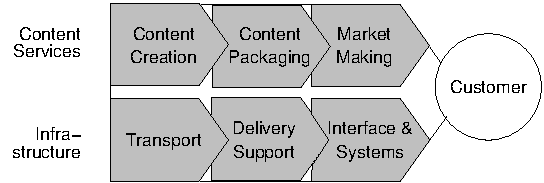
\includegraphics[width=\textwidth]{images/indica_model.pdf}
    \caption{The INDICA two-layered value chain model.}
    \label{fig:indica_model}
  \end{center}
\end{figure}

You can also include JPEG or PNG files, as shown by Figure~\ref{fig:eeyore}.

\begin{figure}[ht]
  \begin{center}
    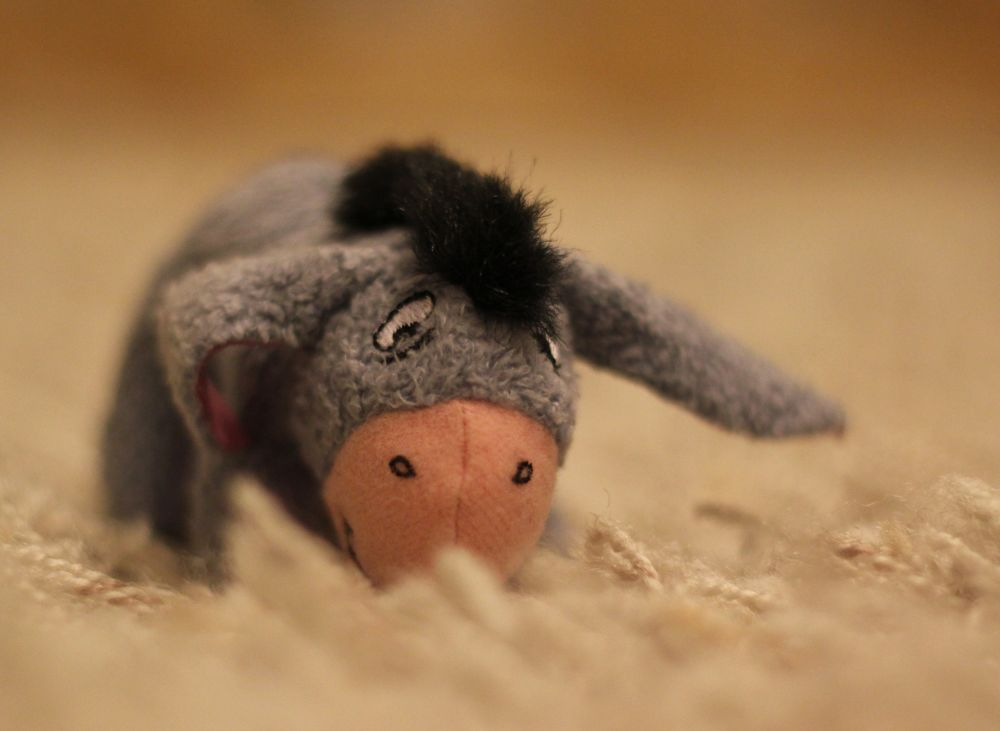
\includegraphics[width=9cm]{images/ihaa.jpg}
    \caption{Eeyore, or Ihaa, a very sad donkey.}
    \label{fig:eeyore}
  \end{center}
\end{figure}

You can create PDF files out of practically anything. 
In Windows, you can download PrimoPDF or CutePDF (or some such) and install a
printing driver so that you can print directly to PDF files from any
application. There are also tools that allow you to upload documents in common
file formats and convert them to the PDF format.
If you have PS or EPS files, you can use the tools \texttt{ps2pdf} or
\texttt{epspdf} to convert your PS and EPS files to PDF\@.

% Comment: If your sentence ends in a capital letter, like here, you should
% write \@ before the period; otherwise LaTeX will assume that this is not
% really an end of the sentence and will not put a large enough space after the
% period. That is, LaTeX assumes that you are (for example), enumerating using
% capital roman numerals, like I. do something, II. do something else. In this
% case, the periods do not end the sentence.

% Similarly, if you do need a normal space after a period (instead of
% the longer sentence separator), use \  (backslash and space) after the
% period. Like so: a.\ first item, b.\ second item.

Furthermore, most newer editor programs allow you to save directly to the PDF
format. For vector editing, you could try Inkscape, which is a new open source
WYSIWYG vector editor that allows you to save directly to PDF\@. 
For graphs, either export/print your graphs from OpenOffice Calc/Microsoft
Excel to PDF format, and then add them; or use \texttt{gnuplot}, which can
create PDF files directly (at least the new versions can).
The terminal type is \emph{pdf}, so the first line of your plot file should be
something like \texttt{set term pdf \ldots}.

To get the most professional-looking graphics, you can encode them using the
TikZ package (TikZ is a frontend for the PGF graphics formatting system).
You can create practically any kind of technical images with TikZ, but it has a
rather steep learning curve. Locate the manual (\texttt{pgfmanual.pdf}) from
your \LaTeX\ distribution and check it out. An example of TikZ-generated
graphics is shown in Figure~\ref{fig:page-merge}.

\begin{figure}[ht]
  \begin{center}
    \newcommand*{\actver}{\smash{\ensuremath{v_{\text{\textit{active}}}}}}

\tikzstyle{lbl}=[font=\scriptsize,midway,sloped]
\tikzstyle{opendash}=[densely dotted,thick] 
\tikzstyle{opendeco}=[decoration={zigzag,amplitude=0.1em,segment length=0.6em}]
\tikzstyle{actverline}=[dashed]
\tikzstyle{entryline}=[densely dotted]
\tikzstyle{area}=[ellipse,draw,dashed]
\tikzstyle{liveentry}=[entryline,postaction={%
  decorate,%
  decoration={%
    markings,%
    mark=at position .5pt with{\arrowreversed[line width=.35pt]{|}};,
    mark=at position 1 with{%
      \arrow[line width=.8pt]{stealth}};%
  }%
}]
\tikzstyle{deadentry}=[entryline,postaction={%
  decorate,%
  decoration={%
    markings,%
    mark=at position .5pt with{\arrowreversed[line width=.35pt]{|}};,
    mark=at position 1 with{%
      \arrow[line width=.8pt]{stealth}};%
%      \arrow[line width=.35pt,black,fill=white]{*}};% 
  }%
}]
\tikzstyle{pageborder}=[thick]
\tikzstyle{pagename}=[anchor=center,text=black!50,font=\huge]
\newlength{\spexx}
\setlength{\spexx}{1.2cm}
\newlength{\spexy}
\setlength{\spexy}{.5cm}

\subfigure[Before]{
\begin{tikzpicture}[x=\spexx,y=\spexy,%
  every pin edge/.style={draw,dotted},%
  pin distance=.5\spexx]
  \small
  \coordinate (lo) at (0,-5);
  \coordinate (o) at (0,0);
  \coordinate (hi) at (0,7);
  \coordinate (loact) at (3,-5);
  \coordinate (oact) at (3,0);
  \coordinate (hiact) at (3,7);
  \coordinate (loinf) at (4,-5);
  \coordinate (oinf) at (4,0);
  \coordinate (hiinf) at (4,7);
  
  \draw[->] (lo) -- node[below,lbl] {Versions} ($(loinf) + (1em,0)$);
  \draw[->] (lo) -- node[above,lbl] {Keys} ($(hi) + (0,1em)$);

  \draw[pageborder] (lo) -- (o) -- (hi);
  \draw[pageborder] (lo) -- (loinf);
  \draw[pageborder] (hi) -- (hiinf);
  \draw[pageborder] (o) -- (oinf);

  \draw[opendash] decorate [opendeco] { (loinf) -- (oinf) };
  \draw[opendash] decorate [opendeco] { (oinf) -- (hiinf) };

  \node[pagename] at (2,3.5) {$p$};
  \node[pagename] at (2,-2.5) {$s$};

  \draw[actverline] ($(loact) + (0,-1em)$) node[below=.4em] {\actver} --
    ($(hiact) + (0,1em)$);

  % Page p contents
  \draw[deadentry] (0,6) -- (1,6);
  \draw[deadentry] (1,6) -- (2,6);
  \draw[deadentry] (2,6) -- (3,6);
  \draw[liveentry] (0,5) -- (4,5);
  \draw[deadentry] (0,4) -- (2,4);
  \draw[deadentry] (1,3) -- (3,3);
  \draw[deadentry] (0,2) -- (1,2);
  \draw[deadentry] (2,2) -- (3,2);
  \draw[deadentry] (0,1) -- (2,1);
  \draw[deadentry] (2,1) -- (3,1);

  % Page s contents
  \draw[liveentry] (0,-1) -- (4,-1);
  \draw[deadentry] (0,-2) -- (2,-2);
  \draw[deadentry] (0,-3) -- (3,-3);
  \draw[liveentry] (3,-4) -- (4,-4);

  \node[area,minimum width=4.5\spexx,minimum height=.6\spexy,pin=178:{$1$}]
    at (2,5) {};
  \node[area,minimum width=4.5\spexx,minimum height=.6\spexy,pin=182:{$2$}]
    at (2,-1) {};
  \node[area,minimum width=1.5\spexx,minimum height=.6\spexy,pin=330:{$3$}]
    at (3.5,-4) {};

\end{tikzpicture}}
\subfigure[After]{
\begin{tikzpicture}[x=\spexx,y=\spexy,%
  every pin edge/.style={draw,dotted},%
  pin distance=.5\spexx]
  \small
  \coordinate (lo) at (0,-5);
  \coordinate (o) at (0,0);
  \coordinate (hi) at (0,7);
  \coordinate (loact) at (3,-5);
  \coordinate (oact) at (3,0);
  \coordinate (hiact) at (3,7);
  \coordinate (loinf) at (4,-5);
  \coordinate (oinf) at (4,0);
  \coordinate (hiinf) at (4,7);

  \draw[->] (lo) -- node[lbl,below] {Versions} ($(loinf) + (1em,0)$);
  \draw[->] (lo) -- node[lbl,above] {Keys} ($(hi) + (0,1em)$);

  \draw[pageborder] (lo) -- (o) -- (hi);
  \draw[pageborder] (lo) -- (loinf);
  \draw[pageborder] (hi) -- (hiinf);
  \draw[pageborder] (o) -- (oact);

  \draw[opendash] decorate [opendeco] { (loinf) -- (oinf) };
  \draw[opendash] decorate [opendeco] { (oinf) -- (hiinf) };

  \node[pagename] at (1.5,3.5) {$p$};
  \node[pagename] at (1.5,-2.5) {$s$};
  \node[pagename] at (3.5,1) {$p'$};

  \draw[actverline] ($(loact) + (0,-1em)$) node[below=.4em] {\actver} -- (loact);
  \draw[pageborder] (loact) -- (hiact);
  \draw[actverline] (hiact) -- ($(hiact) + (0,1em)$);

  % Page p contents
  \draw[deadentry] (0,6) -- (1,6);
  \draw[deadentry] (1,6) -- (2,6);
  \draw[deadentry] (2,6) -- (3,6);
  \draw[deadentry] (0,5) -- (3,5);
  \draw[deadentry] (0,4) -- (2,4);
  \draw[deadentry] (1,3) -- (3,3);
  \draw[deadentry] (0,2) -- (1,2);
  \draw[deadentry] (2,2) -- (3,2);
  \draw[deadentry] (0,1) -- (2,1);
  \draw[deadentry] (2,1) -- (3,1);

  % Page s contents
  \draw[deadentry] (0,-1) -- (3,-1);
  \draw[deadentry] (0,-2) -- (2,-2);
  \draw[deadentry] (0,-3) -- (3,-3);

  % Page p' contents
  \draw[liveentry] (3,5) -- (4,5);
  \draw[liveentry] (3,-1) -- (4,-1);
  \draw[liveentry] (3,-4) -- (4,-4);

  \node[area,minimum width=1.5\spexx,minimum height=.6\spexy,pin=10:{$1$}]
    at (3.5,5) {};
  \node[area,minimum width=1.5\spexx,minimum height=.6\spexy,pin=3:{$2$}]
    at (3.5,-1) {};
  \node[area,minimum width=1.5\spexx,minimum height=.6\spexy,pin=330:{$3$}]
    at (3.5,-4) {};
\end{tikzpicture}}

    \caption{Example of a multiversion database page merge. This figure has
    been taken from the PhD thesis of Haapasalo~\cite{HaapasaloThesis}.}
    \label{fig:page-merge}
  \end{center}
\end{figure}

Another example of graphics created with TikZ is shown in
Figure~\ref{fig:tikz-examples}. 
These show how graphs can be drawn and labeled. 
You can consult the example images and the PGF manual for more examples of what
kinds figures you can draw with TikZ. 

% These definitions are only used in the example images; you will not 
% need them for your thesis...
\newlength{\graphdotsize}
\setlength{\graphdotsize}{1.7pt}
\newlength{\graphgridsize}
\setlength{\graphgridsize}{1.2em}
\begin{figure}[ht]
\begin{center}
\subfigure[Examples of obstruction graphs for the Ferry Problem]{
  \newlength{\oggs}
\setlength{\oggs}{1.2\graphgridsize}
\begin{tikzpicture}[x=\oggs,y=\oggs,every pin edge/.style={draw,dotted},pin distance=0.5\oggs,area/.style={ellipse,draw,dashed}] 

% The graph (0,0,5,0)
% o = origo
\coordinate (o) at (0,0);
\coordinate[left=1 of o,pin=100:$q_1$] (q1);
\coordinate[right=1 of o,pin=80:$q_2$] (q2);
\fill[black] (q1) circle (\graphdotsize);
\fill[black] (q2) circle (\graphdotsize);
\foreach \d in {-2, -1, ..., 2} {
  \coordinate (tmp) at ($(o) + (0,\d)$);
  \draw (q1) -- (tmp);
  \draw (q2) -- (tmp);
  \fill[black] (tmp) circle (\graphdotsize);
}
\node[area,minimum height=5.3\oggs,minimum width=0.8\oggs,pin=94:$X_3$] at (o) {};  

% The graph (1,0,3,0)
\coordinate[right=5 of o] (o);
\coordinate[left=1 of o,pin=260:$q_1$] (q1);
\coordinate[left=2 of o] (q1v);
\coordinate[right=1 of o,pin=280:$q_2$] (q2);
\fill[black] (q1) circle (\graphdotsize);
\fill[black] (q2) circle (\graphdotsize);
\fill[black] (q1v) circle (\graphdotsize);
\draw (q1) -- (q1v);
\foreach \d in {-1, 0, 1} {
  \coordinate (tmp) at ($(o) + (0,\d)$);
  \draw (q1) -- (tmp);
  \draw (q2) -- (tmp);
  \fill[black] (tmp) circle (\graphdotsize);
}
\node[area,minimum height=3.3\oggs,minimum width=0.8\oggs,pin=266:$X_3$] at (o) {};  
\node[area,minimum height=0.8\oggs,minimum width=0.8\oggs,pin=260:$X_1$] at (q1v) {};  


% The graph (0,1,3,0)
\coordinate[right=4 of o] (o);
\coordinate[left=1 of o,pin=100:$q_1$] (q1);
\coordinate[right=1 of o,pin=80:$q_2$] (q2);
\coordinate[right=2 of o] (q2v);
\fill[black] (q1) circle (\graphdotsize);
\fill[black] (q2) circle (\graphdotsize);
\fill[black] (q2v) circle (\graphdotsize);
\draw (q2) -- (q2v);
\foreach \d in {-1, 0, 1} {
  \coordinate (tmp) at ($(o) + (0,\d)$);
  \draw (q1) -- (tmp);
  \draw (q2) -- (tmp);
  \fill[black] (tmp) circle (\graphdotsize);
}
\node[area,minimum height=3.3\oggs,minimum width=0.8\oggs,pin=94:$X_3$] at (o) {};  
\node[area,minimum height=0.8\oggs,minimum width=0.8\oggs,pin=80:$X_2$] at (q2v) {};  

% The graph (0,0,3,1)
\coordinate[right=5 of o] (o);
\coordinate[left=1 of o,pin=260:$q_1$] (q1);
\coordinate[right=1 of o,pin=290:$q_2$] (q2);
\fill[black] (q1) circle (\graphdotsize);
\fill[black] (q2) circle (\graphdotsize);
\draw (q1) -- (q2);
\foreach \d in {-1, 1, 2} {
  \coordinate (tmp) at ($(o) + (0,\d)$);
  \draw (q1) -- (tmp);
  \draw (q2) -- (tmp);
  \fill[black] (tmp) circle (\graphdotsize);
}
\node[area,minimum height=4.3\oggs,minimum width=0.8\oggs,pin=266:$X_3$] at ($(o) + (0,0.5)$) {};  

\end{tikzpicture}

}
\subfigure[Examples of star graphs]{
  \begin{tikzpicture}[x=\graphgridsize,y=\graphgridsize] 

\coordinate (o) at (0,0);
\fill[black] (o) circle (\graphdotsize);
\foreach \d in {0, 90, ..., 270} {
  \coordinate (tmp) at ($(o) + (\d:1.5)$);
  \draw (o) -- (tmp);
  \fill[black] (tmp) circle (\graphdotsize);
}

\coordinate[right=4 of o] (o);
\coordinate (o1) at ($(o) + (0:0.3)$);
\coordinate (o2) at ($(o) + (180:0.3)$);
\fill[black] (o1) circle (\graphdotsize);
\fill[black] (o2) circle (\graphdotsize);
\draw (o1) -- (o2);
\foreach \d in {45, 135, 270} {
  \coordinate (tmp\d) at ($(o) + (\d:1.5)$);
  \draw (o2) -- (tmp\d);
  \fill[black] (tmp\d) circle (\graphdotsize);
}
\draw (o1) -- (tmp45);


\coordinate[right=4 of o] (o);
\coordinate (o1) at ($(o) + (0:0.3)$);
\coordinate (o2) at ($(o) + (180:0.3)$);
\fill[black] (o1) circle (\graphdotsize);
\fill[black] (o2) circle (\graphdotsize);
\draw (o1) -- (o2);
\foreach \d in {45, 135, 270} {
  \coordinate (tmp\d) at ($(o) + (\d:1.5)$);
  \draw (o2) -- (tmp\d);
  \fill[black] (tmp\d) circle (\graphdotsize);
}
\draw (o1) -- (tmp45);
\draw (o1) -- (tmp135);


\coordinate[right=4 of o] (o);
\coordinate (o1) at ($(o) + (0:0.3)$);
\coordinate (o2) at ($(o) + (180:0.3)$);
\fill[black] (o1) circle (\graphdotsize);
\fill[black] (o2) circle (\graphdotsize);
\draw (o1) -- (o2);
\foreach \d in {45, 135, 270} {
  \coordinate (tmp\d) at ($(o) + (\d:1.5)$);
  \draw (o1) -- (tmp\d);
  \draw (o2) -- (tmp\d);
  \fill[black] (tmp\d) circle (\graphdotsize);
}


\coordinate[right=3.5 of o] (o);
\coordinate (o1) at ($(o) + (90:0.3)$);
\coordinate (o2) at ($(o) + (210:0.5)$);
\coordinate (o3) at ($(o) + (330:0.5)$);
\fill[black] (o1) circle (\graphdotsize);
\fill[black] (o2) circle (\graphdotsize);
\fill[black] (o3) circle (\graphdotsize);
\draw (o1) -- (o2);
\draw (o1) -- (o3);
\draw (o2) -- (o3);
\foreach \d in {90, 270} {
  \coordinate (tmp\d) at ($(o) + (\d:1.5)$);
  \draw (o2) -- (tmp\d);
  \draw (o3) -- (tmp\d);
  \fill[black] (tmp\d) circle (\graphdotsize);
}
\draw (o1) -- (tmp90);


\coordinate[right=3 of o] (o);
\coordinate (o1) at ($(o) + (90:0.3)$);
\coordinate (o2) at ($(o) + (210:0.5)$);
\coordinate (o3) at ($(o) + (330:0.5)$);
\fill[black] (o1) circle (\graphdotsize);
\fill[black] (o2) circle (\graphdotsize);
\fill[black] (o3) circle (\graphdotsize);
\draw (o1) -- (o2);
\draw (o1) -- (o3);
\draw (o2) -- (o3);
\foreach \d in {90, 270} {
  \coordinate (tmp\d) at ($(o) + (\d:1.5)$);
  \draw (o2) -- (tmp\d);
  \draw (o3) -- (tmp\d);
  \fill[black] (tmp\d) circle (\graphdotsize);
}
\draw (o1) -- (tmp90);
\draw (o1) -- (tmp270);



\coordinate[right=3.5 of o] (o);
\coordinate (o1) at ($(o) + (18:1.3)$);
\coordinate (o2) at ($(o) + (90:1.3)$);
\coordinate (o3) at ($(o) + (162:1.3)$);
\coordinate (o4) at ($(o) + (234:1.3)$);
\coordinate (o5) at ($(o) + (306:1.3)$);
\foreach \d in {1, 2, ..., 5} {
  \fill[black] (o\d) circle (\graphdotsize);
}
\draw (o1) -- (o2);
\draw (o1) -- (o3);
\draw (o1) -- (o4);
\draw (o1) -- (o5);
\draw (o2) -- (o3);
\draw (o2) -- (o4);
\draw (o2) -- (o5);
\draw (o3) -- (o4);
\draw (o3) -- (o5);
\draw (o4) -- (o5);

\end{tikzpicture}

}
\caption{Examples of graphs draw with TikZ. These figures have been taken from a
course report for the graph theory course~\cite{FerryProblem}.}
\label{fig:tikz-examples}
\end{center}
\end{figure}



\chapter{Applied methods and measurements}
\label{chapter:methods}
In order to be able to discover reliable research data, the research methods must be understood thoroughly. This research study gathers data with a few types of usability methods and they are selected according to their practicality and utility in the research study context. Inquiries are used to study the business process and the process itself is measured from many different aspects and also remote evaluation is utilized to gather data easily from distributed locations. 

Methods are used in different stages of the research to follow the structure of human-centered design principles. The following chapter describes these methods in more detail.  

\texttt{TÄHÄN VÄHÄN LAAJEMMIN}

\section{Remote usability evaluation}
\label{sec:rue}

\texttt{TÄHÄN VOISI ETSIÄ LISÄMATERIAALIA}

There are many ways to implement remote usability evaluation.The data logging approach is being discussed in this paper. In the context of usability, logging means practices for mechanically recording the usage of a system.

Usage data of an application can offer valuable information about users' actions and can therefore be utilized in the process of improving software's usability. Even if logging can not replace the traditional usability methods, it provides many advantages over them.  Logging is automatic, objective and it doesn't require direct observation. The data is gathered from the actual running application. \cite{RefWorks:24}	


\subsection{Evaluation process} 

According to Bateman et al. \cite{RefWorks:24} log-based usability evaluation process consist typically of three stages (see Figure \ref{fig:logging_usability_process}). The first is called \emph{application instrumentation} and in that stage logging capability is added to the application. In other words, instrumentation is a process which determines what data will be logged from the usage of an application. In order to gain useful data, successful decisions in instrumentation stage are crucial. Bateman et al. also assert that if wrong decisions are made and therefore large amount of low-level data has been collected, it might be challenging to interpret and it might not reveal any value. On the other hand, they remark that if only high-level events is logged, internal structures may remain undiscovered. Consequently both, low-level and high-level usage data need to be tracked and logged. Sometimes, when log data doesn't supply enough information for interpretation, contextual information is needed. Generally, it requires a significant amount of effort and vigilance to be able to gather all the essential data to be analyzed. \cite{RefWorks:24}

\begin{figure}[H]
  	\centering
  	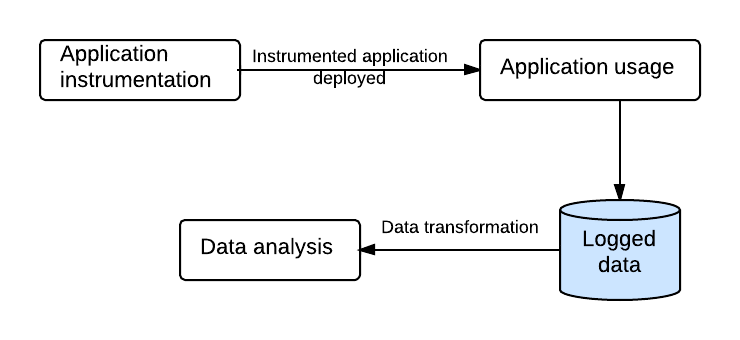
\includegraphics[width=0.8\textwidth]{./images/logging_usability_process.png}
  	\caption{Process for log-based usability evaluation. \cite{RefWorks:24}}
	\label{fig:logging_usability_process}
\end{figure}

The second stage of log-based usability evaluation process is \emph{application usage}. It is a stage where the instrumented application is used in authentic or simulated situation. The log data is collected unobtrusively while the user is performing his tasks with the application. \cite{RefWorks:24}

The final stage of the process is \emph{data analysis}, in which a few different approaches can be used \cite{RefWorks:24, RefWorks:25}:
\begin{itemize}
  \item Synchronize and searching
  \item Transforming event streams
  \item Performing counts and summary statistics
  \item Detecting, comparing and characterizing sequences 
  \item Visualizing
\end{itemize}
This part of the process will be described in more detail in the following subsection \nameref{sec:analysis}.



\subsection{Log data analysis}
\label{sec:analysis}
 In order to gain beneficial usability information from user interface events, the log data has to be analyzed thoroughly. According to  Hilbert and Redmiles \cite{RefWorks:25}, there are several approaches to sort out important usability information out of log data and to make it more understandable for humans.
The first one of them is called \textbf{\emph{synchronization and searching}}. 

It is often challenging to interpret user interface events alone and thereby discover valuable higher level events without any contextual information. The purpose of the synchronization and searching is to combine user interface event data with other informative data, such as observations or video recordings, in order to increase the understanding about the context of use. These two forms of data are complementary and can together provide wider understanding about the usability of a system. Observations or video recordings may supply additional information about the user interface event appeared in the log, or vice versa. However, there are few disadvantages with synchronization and searching techniques. For example video recording and observation typically require the presence of the observer. Furthermore, using video recording as a part of evaluation, produces a lot of data and can be inefficient to analyze. It might also have an disturbing affect on user's behavior. \cite{RefWorks:25}

The second approach is \textbf{\emph{transformation}}. Transformations combine selection, abstraction and recording to transform events into more beneficial form of information. This information can then be utilized for instance in detecting, comparing or characterizing human behavior patterns. Selection is basically segregating useful information out of mass of user interface related events by filtering out irrelevant data or by selecting the relevant data. Example of selection could be a situation where the user has been writing a lot of text, generating a lot of data in the log, and trying to find save button from different menus. From the usability point of view, text inputs as log events are probably not that relevant, but time consuming browsing between different menus can be a sign from usability issues. \cite{RefWorks:25}

Abstraction can be used to combine different events into a more understandable event sequences or patterns. For example user typing into different text fields and then clicking a button in a web page could be interpreted as a login activity. However, in this kind of situation user interface event logs, must be supplemented with contextual data to be assured that the event sequence is really what it appears to be. Recording means generating new sets of events based on selection and abstraction. Less effort is required to analyze new sets of raw data because earlier analyzing techniques can be exploited. \cite{RefWorks:25}

The third way of generating tangible usability information out of user interface log data is to use \textbf{\emph{counts and summary statistics}}. Counts and summary statistics are calculations based on usability-related metrics gathered from the log data. For instance, calculating the time spent on a specific task (performance time),  can be critical information in usability evaluation. \cite{RefWorks:24, RefWorks:25}

\textbf{\emph{Detecting, comparing and characterizing sequences}} are approaches which utilize sequence information of events. Sequence detection refers to an action in which ready-defined sequences are tried to be identified from the mass of source sequences. Sequence comparison is  executed by usability analyst and it is made between two sequences. These two sequences can be generated for example by subjects or subject groups. In any case, the purpose of sequence comparison is to compare actual usage against some defined ideal usage. Sequence characterization uses the source sequences to create a model to summarize all features of interest in those source sequences. \cite{RefWorks:24, RefWorks:25}
 
The last approach for log-based data analysis is called \textbf{\emph{visualization}}. In visualization, transformed and analyzed data is  presented in a graphical form. General way to visualize data is to use charts, but it is possible to use other visualization techniques such as heat maps based on clicks or mouse traveling. \cite{RefWorks:24, RefWorks:25}

\section{Contextual Inquiry}
\label{sec:cinquiry}
\texttt{TÄHÄN VIELÄ p1-raven pdfstä juttua.}
Contextual Inquiry is an unstructured interview method, but it has some qualities which differs it from traditional unstructured interviews.\cite{RefWorks:23}  It was originally developed to meet three requirements. Firstly it was supposed to identify a design process for systems that will be used similarly in different business contexts and in different cultures. It was also supposed to identify a convenient process for gathering user information in limited time and finally to identify a way to acquire information about users' work in eligible format. In addition to those requirements, the technique was noticed to be capable of much more. CI cherish participatory design and, because of that quality, users are able to involve in the design. Users' contributes to the design by providing a deep understanding about the nature of the work. This is done through inquiry and it's a basis for fundamental work concepts. \cite{RefWorks:14} 

\subsection{Fundamentals of Contextual Inquiry}
Contextual Inquiry can be said to be an apprenticeship compressed in time. The basis of the method is premised on the idea of user being the expert instead of the interviewer, but unlike an apprentice, the interviewer neither learns the work by doing it, nor has the same amount of time available for learning. \cite{RefWorks:21} CI differs from the traditional master-apprenticeship model in other ways also. A few fundamental principles of Contextual Inquiry are said to be essential in order to meet the specific needs of design problems \cite{RefWorks:21, RefWorks:22}.  These principles are understanding the context of the work, creating a partnership, interpreting the work and steering the focus during the interview. \cite{RefWorks:21}

Understanding the \textbf{context} of the work is the baseline of Contextual Inquiry. To gain the understanding about the work structure, the interviewer must pursue understanding about the details of users' work and these details can be found by following the users' actions at work. In general, it is important that interviewer avoids gathering abstract or summarized information about the context.\cite{RefWorks:21}

It is essential to create collaborative environment and a \textbf{partnership} between the user and the interviewer while the real life work structure and activities are tried to be understood thoroughly. Partnership is an equal relationship between the interviewer and the user. In comparison to traditional interview or master-apprentice approaches, partnership doesn't give any power advantage to either parties. Instead, it fosters the interviewer's expertise to see the work structure and the user's expertise to do the work. There are many advantages in partnership approach. For example by paying attention to details and structure of work, interviewer can also teach the user to attend to them. In the best case scenario the interviewer and the user watch the work structure and think about design possibilities together. In this kind of scenario it is common that the work is suspended, while the parties discuss about the work structure, and then return again. For interviewer asking feedback for design ideas is also encouraged.\cite{RefWorks:21}

Even if a partnership should be created between the parties, the interviewer should still be able to steer the interview and keep the \textbf{focus} of the conversation on work-related topics relevant to the design \cite{RefWorks:21}. The focus point should be decided before the research takes place, and data gathering should have a deliberated and precise goal. This goal or focus should be dependent on the information needs of the design.\cite{RefWorks:22}

The success of Contextual Inquiry and system design depends on the facts gathered, but the facts are not enough. They are a starting point.\textit{"From the fact, the observable event, the designers makes a hypothesis, an initial interpretation about what the fact means or the intent behind the fact."}\cite{RefWorks:21} In other words, \textbf{interpretations} are needed and they are critical for success. In the final version of the system, interpretations have to be correct or the system fails. This is why it is important to share and validate the interpretations with the customer early enough. \cite{RefWorks:21}

As soon as thorough understanding about the work is available, design for a system model can be created.\cite{RefWorks:14} 

\subsection{Contextual Inquiry interviews}

Practical preparations of CI includes careful planning. The first phase of planning is to set the focus for the research. Focus can be for example a definition of a problem which need to be solved. It creates ground rules for the interview and it is therefore easier for the interviewer to steer the conversation. After the focus has been set, the inquiry itself need to be designed. The challenge in inquiry design is to find a way to determine underlying issues which cause problems in the work. The approach for the design should be slightly different if the aim of the Contextual Inquiry is to support upgrading the system, creating a totally new system or redesigning the process. If CI is used to help the design process of a new system, a challenge is to get the designers and the users to work together in order to define new ways of working, and to develop a system design to support them. \cite{RefWorks:21} 

The structure of the interview is considerably straightforward. First task of the interviewer is to introduce the CI process and ask permission to record the conversation and the work. The interviewer has to also make it clear that understanding the work of the user is the primary target of the research, and that all the misunderstandings should be corrected. This is called the conventional interview phase. The next step of the interview is to clarify the rules. In traditional Contextual Inquiry process it is desirable for the interviewer to interrupt and ask questions and correspondingly for the user to indicate if the time is inconvenient for interruption. This phase is called a transition. The third part of the CI is the actual interview (the contextual interview proper phase), which consist of observation, asking direct questions, suggesting interpretations, writing notes and recording the whole chain of events. Finally the interviewer should wrap up (the wrap-up phase) the interview, ensure that everything is understood correctly and summarize the process. This is the last chance for the user to revise misunderstandings. \cite{RefWorks:21}

Contextual Inquiry is usually conducted by one person and the interviewee. If two people are used, the roles of note-taker and interviewer must be separated. This means that interviewer is leading the discussion and the note-taker does not involve in it. The approximate length of the interview should be two hours. It is also important to get an overview of user's background and demographic information in order to be able to focus on relevant things. It is also important \emph{not to use predefined set of questions}, but to familiarize oneself  with the ares of concern in the process. Artifacts offering relevant information about the work, such as cheat sheets or notes, should be also collected, photographed or copied. \cite{RefWorks:27} Reviewing the notes is usually required after the interview in order to ensure their comprehensiveness. It is probable that some ideas or impressions might have forgotten during the interview. \cite{RefWorks:28}


\subsection{Analysing the data}

The data gathered from Contextual Inquiry consist of notes, recordings and possibly artifacts. In order to be able to analyze the data, it has to be in identical format. This is why it might be beneficial to create a summation of the data. It can be done for example by transcribing important notes from the recordings and by describing the artifacts and their use. Once the data is coherent, the analysis can begin. 

The analysis of CI consist of three steps. The first step is to set focus for the analysis. It is often the same than for the inquiry itself, but occasionally insights from the inquiry makes the original focus outdated. In this case, the new focus for the analysis need to be identified. The next phase in CI analysis is to choose the data display. There are various of methods available for that, such as affinity and workflow diagrams. After the data display has been chosen the final step is to organize the data in the data display. \cite{RefWorks:28}

The affinity diagram organizes single notes in to higher categories or hierarchies. In affinity diagram there are no predefined categories for the individual notes. Instead, a single note is being used to define a category and then the corresponding notes are being attached to the same category. In other words, the notes creates categories and categories then raises common structures and themes. After the categories or groups are formed, and there is no floating notes left, the groups have to be descriptively named. Then groups of groups are being collected, and thereby hierarchies created. The named groups and hierarchies, and the headings of them, then represents new information in an affinity. \cite{RefWorks:21, RefWorks:28}

The workflow diagram can be used if the work process need to be tracked and understood thoroughly. At first, the notes from each interview need to be reviewed, after which the flow charts can be conducted. The flow charts should reflect the work process of each individual in every interview. After that all the flowcharts need to be displayed and compared. Finally, a composite work flow diagram (containing the stages perceived in most of the inquiries) can be created. \cite{RefWorks:28}

\section{Cognitive Walkthrough}
\label{sec:cognitivewalkthrough}

Cognitive Walkthrough (CW) was developed in the early nineties and it was originally intended to help reviewing 'walk-up-and-use' interfaces, such as Automatic Teller Machine (ATM). CW is a formal usability inspection method for professionals involved in the development process. The key concept behind CW is to use theory as a guide for design review. It is easy to understand and apply and therefore feasible to use in a regular development process. \cite{RefWorks:19, RefWorks:18} 
The method consist of two phases: preparatory and analysis phases. In the preparatory phase, the tasks, sequences for tasks, users and their backgrounds and the interface to be analyzed will be agreed upon.  The actual analysis will be accomplished in the analysis phase, where every action of every task will be executed and analyzed. In general the Cognitive Walkthrough method can benefit all phases of the design and development process.\cite{RefWorks:26}

\subsection{Preparations}
Cognitive Walkthrough can be accomplished by using detailed design specification of the user interface which has been received after requirement analysis and functionality definition processes. The walkthrough can be also performed  on a paper simulation, minimal prototype or fully functional prototype of the UI. Formally Cognitive Walkthrough evaluates design's ease of learning by exploring it. \cite{RefWorks:26}

The analysis can be done individually or in a group. In a group the process starts with designers presenting the design to a group of peers and it's usually done after a certain milestone in interface design. The designers can then benefit from the feedback and improve the implementation for the next revision. Participants may represent different organizational units and in the evaluation team they have to adopt different roles, such as recorder, facilitator and various kinds of expert roles. \cite{RefWorks:26}

The first step in walkthrough preparations is to describe the users of the system and choose the tasks for analysis. If the background and technical experience of the users are described in the beginning, more details can be possibly revealed in the walkthrough itself. The selection of tasks (for analysis) is critical and should be based on facts, such as requirement analysis, needs analysis or concept testing. The amount of tasks should be moderate and it is important that the set of chosen tasks include some core functionality and some combinations between those core functionalities. Furthermore, to make tasks as concrete as possible, context descriptions must be included. \cite{RefWorks:26}

After the tasks have been chosen,  the action sequences for the tasks need to be described. Basically it means that the sequence of actions, which are required to accomplish the task with the UI, are being described. These actions can be as simple as "press the start button" or "write your name in the text field". However, depending on the level of user expertise and user descriptions, actions might also consist of several simple actions which can then be executed as one block. These kind of actions could be for example filling in the register form or going to a specific website. The interface definition should include the prompts preceding all the actions in the task and the interface's reactions to those actions. If the development is already finished, all the information from the interface is available, but if the development process is only in the beginning, paper descriptions are needed. The level of detail in paper descriptions depend once again on the expertise of the users. \cite{RefWorks:26}

\subsection{Analysis}

The Contextual Inquiry analysis phase examines the actions of the tasks and generates a plausible story or a review about the reasons why the users (which have been defined earlier) would have chosen those actions. These stories are based on presumptions about user's expertise and objectives. Sometimes users trust on their problem-solving skills, which is why it is important to understand the problem-solving process in the analysis phase. In order to mimic this process in the analysis phase, four steps should be taken. First, a rough description of the task to be accomplished should be considered. Then the user interface should be explored and actions should be taken according to assumptions users might have. The third step is to observe if the user interface is returning the expected results for each action. The last part of problem-solving process is to assume and define users' next action.\cite{RefWorks:26}

\texttt{TÄHÄN VIELÄ LISÄÄ ARTIKKELISTA + ETSI MUUTA AINEISTOA}

\section{Interaction Sequence Illustration}
\label{sec:isi}
Considering the practical impacts of the thesis, it is important to use methods and measures which can shore up the software development process in a real-use context. This is why the process and it's interactions are reviewed using ISI method, which utilizes 				authentic use context and real users. \cite{RefWorks:17} ISI was originally developed for evaluating the usability of IT tasks carried out in healthcare industry, but there are no defined reasons why it could not be utilized in different environments.

\subsection{Description of the Interaction Sequence Illustration}
Interaction Sequence Illustration is a low level analysis method for human-computer interaction. It uses data acquired during the Contextual Inquiry process and doesn't gather any of its own. However, the inquiry data has to be complemented with documentation 			about 	interaction activities. There are three objectives for ISI method to handle. The first is to demonstrate how the user perceives the system. The second one is to identify and document activities, and to discover problems. The first two objectives creates the 			third one, which is to support the user-centered design and development. \cite{RefWorks:17}  The strength of ISI lies in the analysis of data and it can be used to compare the interaction sequences of two of or more UI implementations. On the other hand it can 			provide prominent information on only one UI's interaction sequence. 

\subsection{Utilization of the Interaction Sequence Illustration}
The utilization of Interaction Sequence Illustration can be simplified in seven steps (see Figure \ref{fig:isi_chart}). First the data need to be collect (notes and screenshots) alongside Contextual Inquiry interview.
Then the screenshots need to be arranged in the right order and all the superfluous data need to be removed. The third phase is to count the interaction steps based on screenshots and activity analysis.
After the analysis the screenshots needs to be modified and important details highlighted. Then the sequence numbers as well as a  detailed description text should be added to give a profound understanding about the actions. The outcomes of the method are 			illustration, or illustrations depending on the number of research objectives, of the interaction stages. Every stage contains step-by-step illustration (or illustrations) of user-computer interaction. \cite{RefWorks:17}
	
\begin{figure}[H]
  	\centering
  	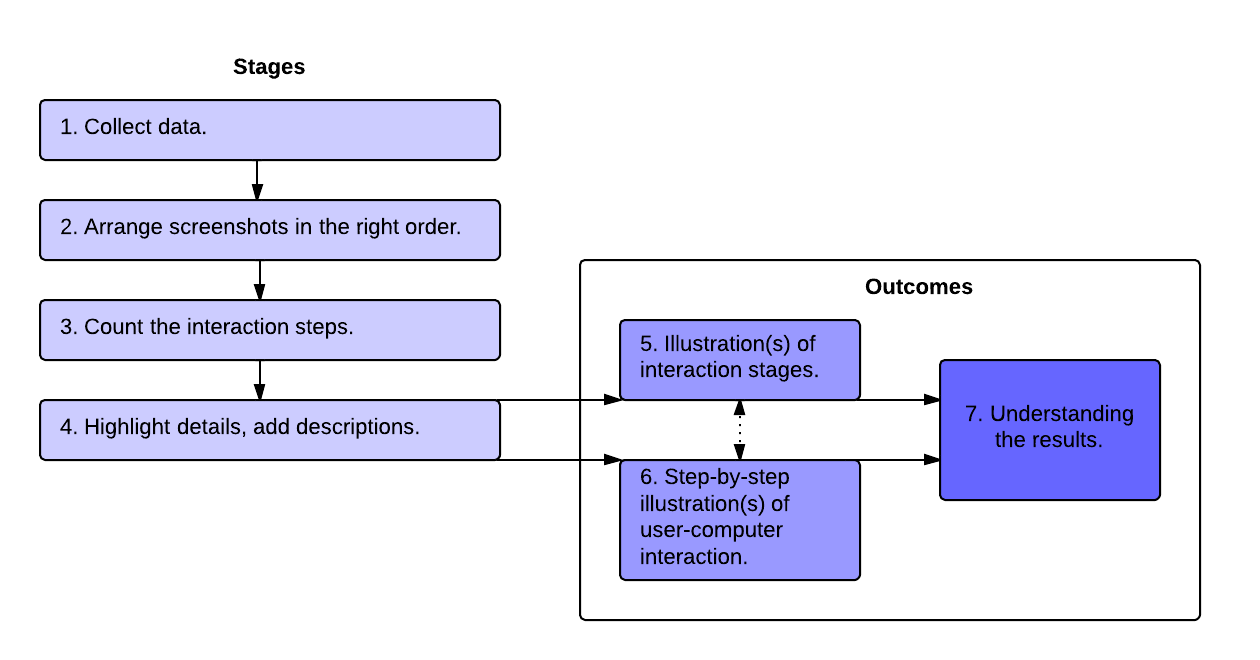
\includegraphics[width=1.1\textwidth]{./images/isi_chart.png}
  	\caption{Interaction Sequence Illustration steps and outcomes.}
	\label{fig:isi_chart}
\end{figure}

\section{System Usability Scale}
\label{sec:sus}
In his paper Brooke \cite{RefWorks:10} argued that usability is not any real existing quality, but a good usability artifact is \emph{appropriate to its purpose}. In other words "the usability of any tool or system has to be viewed in terms of the context in which it is 			used, and its appropriateness to that context"\cite{RefWorks:10}. Still in many cases, context related usability evaluation is not desirable. The reason for this is that a large scale context analysis is usually neither cost-efficient nor practical.\cite{RefWorks:10} 
SUS responds to these challenges by offering an easy and quick way to get subjective ratings about the usability of a system. It is not limited to any specific technology, which makes it universal tool for usability evaluation. \cite{RefWorks:12}

\subsection{Description of the System Usability Scale}
System Usability Scale (see \nameref{app:susform}) is a ten-item \emph{Likert scale}, meaning that every item consist of the scale of five, ranging from "Strongly disagree" to "Strongly agree". The questionnaire is generally being filled right after the possibility to use 		the system to be evaluated. The focus should be on immediate responses and too much time shouldn't be given to the respondents. \cite{RefWorks:10} 
\texttt{TÄHÄN LISÄÄ!!! TEN YEARS OF SUS -ARTIKKELISTA}


\subsection{System Usability Scale in practice}
The outcome of SUS is a single value which express the overall usability of the system. The value consist of all the items and none of them are meaningful as such. System Usability Scale can be calculated by first summing the score contribution (range from 0 to 4) 			from each item. Before summing the scale positions of the items 1,3,5,7 and 9 need to be subtracted by one and the scale positions of the items 2,4,6,8 and 10 need to be subtracted from 5. The last step is to multiply the sum of the scores by 2.5 to get the overall 			SUS value, which will range from minimum of 0 to maximum of 100. \cite{RefWorks:10} The resulting single score is an easy-to-understand measure, and can therefore be discussed with the wide range of stakeholders. \cite{RefWorks:12} 

	

\section{Quantitative measurements in usability evaluation}
\label{sec:other}
The last process measurements used in the research are simply the time which was consumed while carrying out the task and the success rate of the task.


 
    
\chapter{Usability evaluation experiment}
\label{experiment}

Human-centered design consist a few activities and iterative process (see Figure \ref{fig:hci_process}). \cite{RefWorks:16} The empirical part of this thesis adapts human-centered design principles and the steps of the process experiment are highly linked to its activities. The reasoning for this approach in the pragmatical part of the research study can be found from the earlier research done about the topic. \texttt{miksi hyvä???} 
The steps are described in detail in section \ref{sec:dprocess}. This chapter will also describe the implementation phases of the experiment. 

\texttt{TÄHÄN JOTAIN CONTEXTUAL DESIGNISTÄ JA ITSE PROSESSISTA JOTA ARVIOIDAAN!!!!!}

\begin{figure}[H]
  	\centering
    	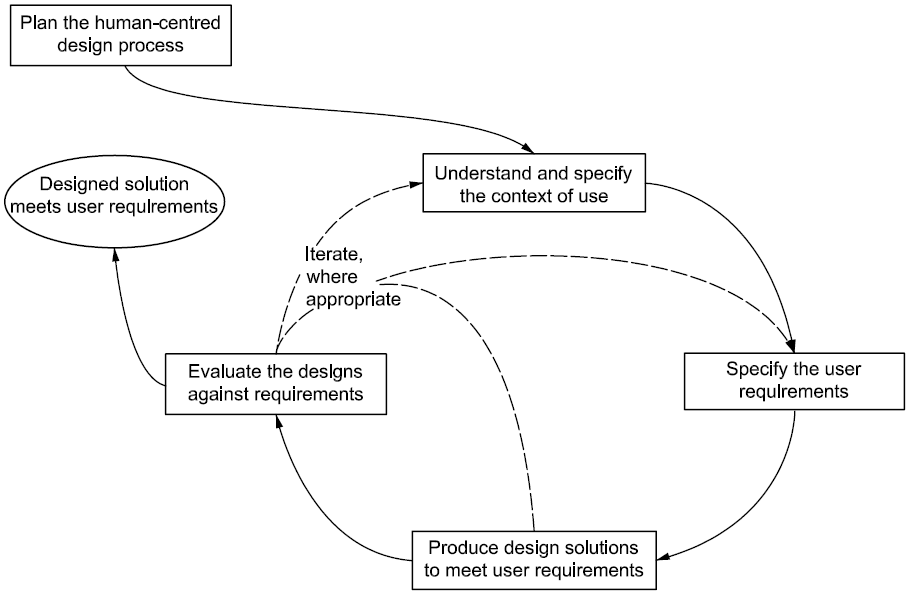
\includegraphics[width=1.0\textwidth]{./images/hci_process.png}
  	\caption{Human-centered design activities.\cite{RefWorks:16}}
	\label{fig:hci_process}
\end{figure}

\section{Applied human-centered design process}
\label{sec:dprocess}

This part of the thesis forms the first step of the human-centered design process: \emph{Planning the design process}. The section applies the framework of the human-centered design process and offers one possible approach to user-centered in-house software development.

The process itself is executed by the personnel highly expertized in the area of customer service and the primary tool for the process is a tailored ERP system. Moreover, the distinctive nature of the business sets additional challenges for the usability evaluation. This is why it is presumable that the process can not be understood thoroughly without understanding the work in practice. Because of the reasons mentioned earlier, Contextual Inquiry is chosen as a method for \emph{understanding and specifying the context of use}. 

The researcher must have a profound understanding about the context of use in order to \emph{specify the user requirements}. A qualified system can be implemented only if the user requirements are precisely defined. Many of the methods used in this experiment aims to assist in this crucial state of development. Technically the process of requirement specification can be initiated while running the Contextual Inquiry. Although, it is essential to remember that the focus in CI should be mostly on understanding the context of use. This thesis uses user evaluation, expert evaluation and measurement methods to identify all the user requirements affecting on the user experience and the functionality of the system.

While the user requirements have been specified, \emph{design solution can be produced according to these requirements}. 


        \begin{itemize}
            \item Creating the model for gathering data
            \item Modified contextual inquiry 
            \item Process measurement methods
            \item Analysis 1.
            \item Prototype creation
            \item Remote evaluation - process measurement methods.
            \item Analysis 2.
        \end{itemize}

    \section{Practical implementation}
    \label{sec:implementation}
    
	\texttt{Kuinka monta osallistujaa, millainen ympäristö, missä maassa, minkä ikäisiä osallistujat, kauanko tehneet työtä}
    	\texttt{kuinka testaus sujui, menetelmäkohtaisesti, mitä välineitä käytettiin miten toimi.}
    	
\chapter{Analysis}
\label{chapter:analysis}

    \section{Results and comparisons}
    \label{sec:results}
    -Comparison between country offices
    -Comparison between individuals (esim. kuinka kauan kesti tietyn toiminnon tekeminen) / Overall comparison (esim. kaikkien koehenkilöiden yhteinen kehitys.)
- Interaction sequence illustration (esim. kuinka monta steppiä ennen ja jälkeen)

    \section{Implementation analysis}
    \label{sec:implementationanalysis}
    -Should these methods be implemented as a part of the process or not.

%When you use \texttt{pdflatex} to render your thesis, you can include PDF images
%directly, as shown by Figure~\ref{fig:indica_model} below.

%\begin{figure}[ht]
%  \begin{center}
%    \includegraphics[width=\textwidth]{example_indica_model.pdf}
%    \caption{The INDICA two-layered value chain model.}
%    \label{fig:indica_model}
%  \end{center}
%\end{figure}

%You can also include JPEG or PNG files, as shown by Figure~\ref{fig:eeyore}.

%\begin{figure}[ht]
%  \begin{center}
%    \includegraphics[width=9cm]{example_ihaa.jpg}
%    \caption{Eeyore, or Ihaa, a very sad donkey.}
%    \label{fig:eeyore}
%  \end{center}
%\end{figure}


%If you have PS or EPS files, you can use the tools \texttt{ps2pdf} or
%\texttt{epspdf} to convert your PS and EPS files to PDF\@.

% Comment: If your sentence ends in a capital letter, like here, you should
% write \@ before the period; otherwise LaTeX will assume that this is not
% really an end of the sentence and will not put a large enough space after the
% period. That is, LaTeX assumes that you are (for example), enumerating using
% capital roman numerals, like I. do something, II. do something else. In this
% case, the periods do not end the sentence.

% Similarly, if you do need a normal space after a period (instead of
% the longer sentence separator), use \  (backslash and space) after the
% period. Like so: a.\ first item, b.\ second item.


%WYSIWYG vector editor that allows you to save directly to PDF\@.

%Excel to PDF format, and then add them; or use \texttt{gnuplot}, which can
%something like \texttt{set term pdf \ldots}.


%rather steep learning curve. Locate the manual (\texttt{pgfmanual.pdf}) from
%graphics is shown in Figure~\ref{fig:page-merge}.

%\begin{figure}[ht]
%  \begin{center}
%    \input{example_page-merge.tex}
%    \caption{Example of a multiversion database page merge. This figure has
%    been taken from the PhD thesis of Haapasalo~\cite{HaapasaloThesis}.}
%    \label{fig:page-merge}
%  \end{center}
%\end{figure}


% These definitions are only used in the example images; you will not
% need them for your thesis...
%\newlength{\graphdotsize}
%\setlength{\graphdotsize}{1.7pt}
%\newlength{\graphgridsize}
%\setlength{\graphgridsize}{1.2em}
%\begin{figure}[ht]
%\begin{center}
%\subfigure[Examples of obstruction graphs for the Ferry Problem]{
%  \input{example_obstruction-grouped.tex}
%}
%\subfigure[Examples of star graphs]{
%  \input{example_general-star-graphs.tex}
%}
%\caption{Examples of graphs draw with TikZ. These figures have been taken from a
%course report for the graph theory course~\cite{FerryProblem}.}
%\label{fig:tikz-examples}
%\end{center}
%\end{figure}



% \chapter{Methods}
\label{chapter:methods}

You have now stated your problem, and you are ready to do something
about it!  \emph{How} are you going to do that? What methods do you
use?  You also need to review existing literature to justify your
choices, meaning that why you have chosen the method to be applied in
your work.

% An example of a traditional LaTeX table
% ------------------------------------------------------------------
% A note on underfull/overfull table cells and tables:
% ------------------------------------------------------------------
% In professional typography, the width of the text in a page is always a lot
% less than the width of the page. If you are accustomed to the (too wide) text
% areas used in Microsoft Word's standard documents, the width of the text in
% this thesis layout may suprise you. However, text in a book needs wide
% margins. Narrow text is easier to read and looks nicer. Longer lines are 
% hard to read, because the start of the next line is harder to locate when
% moving from line to the next. 
% However, tables that are in the middle of the text often would require a wider
% area. By default, LaTeX will complain if you create too wide tables with
% ``overfull'' error messages, and the table will not be positioned properly
% (not centered). If at all possible, try to make the table narrow enough so
% that it fits to the same space as the text (total width = \textwidth).
% If you do need more space, you can either
% 1) ignore the LaTeX warnings 
% 2) use the textpos-package to manually position the table (read the package
%    documentation)
% 3) if you have the table as a PDF document (of correct size, A4), you can use
%    the pdfpages package to include the page. This overrides the margin
%    settings for this page and LaTeX will not complain.
% ------------------------------------------------------------------
% Another note:
% ------------------------------------------------------------------
% If your table fits to \textwidth, but the cells are so narrow that the text
% in p{..}-formatted cells does not flow nicely (you get underfull warnings 
% because LaTeX tries to justify the text in the cells) you can manually set
% the text to unjustified by using the \raggedright command for each cell 
% that you do not want to be justified (see the example below). \raggedleft 
% is also possible, of course...
% ------------------------------------------------------------------
% If you need to have linefeeds (\\) inside a cell, you must create a new
% paragraph-formatting environment inside the cell. Most common ones are 
% the minipage-environment and the \parbox command (see LaTeX documentation
% for details; or just google for ``LaTeX minipage'' and ``LaTeX parbox'').
\begin{table}
\begin{tabular}{|p{2cm}|p{3.8cm}|p{4.5cm}|p{1.1cm}|} 
% Alignment of sells: l=left, c=center, r=right. 
% If you want wrapping lines, use p{width} exact cell widths.
% If you want vertical lines between columns, write | above between the letters
% Horizontal lines are generated with the \hline command:
\hline % The line on top of the table
\textbf{Code} & \textbf{Name} & \textbf{Methods} & \textbf{Area} \\ 
\hline 
% Place a & between the columns
% In the end of the line, use two backslashes \\ to break the line,
% then place a \hline to make a horizontal line below the row 
T-110.6130 & Systems Engineering for Data Communications
    Software & \raggedright Computer simulations, mathematical modeling,
  experimental research, data analysis, and network service business
  research methods, (agile method) & T-110 \\ 
\hline
\multicolumn{2}{|p{6.25cm}|}{Mat-2.3170 Simulation (here is an example of
 multicolumn for tables)}& Details of how to build simulations & T-110 \\
% The multicolumn command takes the following 3 arguments: 
% the number of cells to merge, the cell formatting for the new cell, and the
% contents of the cell
\hline
S-38.3184 & Network Traffic Measurements and Analysis 
& \raggedright How to measure and analyse network
  traffic & T-110 \\ \hline
\end{tabular} % for really simple tables, you can just use tabular
% You can place the caption either below (like here) or above the table
\caption{Research methodology courses}
% Place the label just after the caption to make the link work
\label{table:courses}
\end{table} % table makes a floating object with a title

If you have not yet done any (real) metholodogical courses (but chosen
introduction courses of different areas that are listed in the
methodological courses list), now is the time to do so or at least
check through material of suitable methodological courses. Good
methodologial courses that consentrates especially to methods are
presented in Table~\ref{table:courses}. Remember to explain the
content of the tables (as with figures). In the table, the last column
gives the research area where the methods are often used. Here we used
table to give an example of tables. Abbreviations and Acronyms is also
a long table. The difference is that longtables can continue to next
page.




% An example of a traditional LaTeX table
% ------------------------------------------------------------------
% A note on underfull/overfull table cells and tables:
% ------------------------------------------------------------------
% In professional typography, the width of the text in a page is always a lot
% less than the width of the page. If you are accustomed to the (too wide) text
% areas used in Microsoft Word's standard documents, the width of the text in
% this thesis layout may suprise you. However, text in a book needs wide
% margins. Narrow text is easier to read and looks nicer. Longer lines are
% hard to read, because the start of the next line is harder to locate when
% moving from line to the next.
% However, tables that are in the middle of the text often would require a wider
% area. By default, LaTeX will complain if you create too wide tables with
% ``overfull'' error messages, and the table will not be positioned properly
% (not centered). If at all possible, try to make the table narrow enough so
% that it fits to the same space as the text (total width = \textwidth).
% If you do need more space, you can either
% 1) ignore the LaTeX warnings
% 2) use the textpos-package to manually position the table (read the package
%    documentation)
% 3) if you have the table as a PDF document (of correct size, A4), you can use
%    the pdfpages package to include the page. This overrides the margin
%    settings for this page and LaTeX will not complain.
% ------------------------------------------------------------------
% Another note:
% ------------------------------------------------------------------
% If your table fits to \textwidth, but the cells are so narrow that the text
% in p{..}-formatted cells does not flow nicely (you get underfull warnings
% because LaTeX tries to justify the text in the cells) you can manually set
% the text to unjustified by using the \raggedright command for each cell
% that you do not want to be justified (see the example below). \raggedleft
% is also possible, of course...
% ------------------------------------------------------------------
% If you need to have linefeeds (\\) inside a cell, you must create a new
% paragraph-formatting environment inside the cell. Most common ones are
% the minipage-environment and the \parbox command (see LaTeX documentation
% for details; or just google for ``LaTeX minipage'' and ``LaTeX parbox'').
%\begin{table}
%\begin{tabular}{|p{2cm}|p{3.8cm}|p{4.5cm}|p{1.1cm}|}
% Alignment of sells: l=left, c=center, r=right.
% If you want wrapping lines, use p{width} exact cell widths.
% If you want vertical lines between columns, write | above between the letters
% Horizontal lines are generated with the \hline command:
%\hline % The line on top of the table
%\textbf{Code} & \textbf{Name} & \textbf{Methods} & \textbf{Area} \\
%\hline
% Place a & between the columns
% In the end of the line, use two backslashes \\ to break the line,
% then place a \hline to make a horizontal line below the row

%    Software & \raggedright Computer simulations, mathematical modeling,

%\hline
%\multicolumn{2}{|p{6.25cm}|}{Mat-2.3170 Simulation (here is an example of
% multicolumn for tables)}& Details of how to build simulations & T-110 \\
% The multicolumn command takes the following 3 arguments:
% the number of cells to merge, the cell formatting for the new cell, and the
% contents of the cell
%\hline
%S-38.3184 & Network Traffic Measurements and Analysis
%& \raggedright How to measure and analyse network
%  traffic & T-110 \\ \hline
%\end{tabular} % for really simple tables, you can just use tabular
% You can place the caption either below (like here) or above the table
%\caption{Research methodology courses}
% Place the label just after the caption to make the link work
%\label{table:courses}
%\end{table} % table makes a floating object with a title



% \chapter{Implementation}
\label{chapter:implementation}

You have now explained how you are going to tackle your problem. 
Go do that now! Come back when the problem is solved!

Now, how did you solve the problem? 
Explain how you implemented your solution, be it a software component, a
custom-made FPGA, a fried jelly bean, or whatever.
Describe the problems you encountered with your implementation work.




% \chapter{Evaluation}
\label{chapter:evaluation}

You have done your work, but that's\footnote{By the way, do \emph{not} use
shorthands like this in your text! It is not professional! Always write out all
the words: ``that is''.} not enough. 

You also need to evaluate how well your implementation works.  The
nature of the evaluation depends on your problem, your method, and
your implementation that are all described in the thesis before this
chapter.  If you have created a program for exact-text matching, then
you measure how long it takes for your implementation to search for
different patterns, and compare it against the implementation that was
used before.  If you have designed a process for managing software
projects, you perhaps interview people working with a waterfall-style
management process, have them adapt your management process, and
interview them again after they have worked with your process for some
time. See what's changed.

The important thing is that you can evaluate your success somehow.
Remember that you do not have to succeed in making something spectacular; a
total implementation failure may still give grounds for a very good master's
thesis---if you can analyze what went wrong and what should have been done.

 




%You have done your work, but that's\footnote{By the way, do \emph{not} use







% \chapter{Discussion}
\label{chapter:discussion}

At this point, you will have some insightful thoughts on your implementation
and you may have ideas on what could be done in the future. 
This chapter is a good place to discuss your thesis as a whole and to show your
professor that you have really understood some non-trivial aspects of the
methods you used\ldots



\chapter{Summary and conclusions}
\label{chapter:summary}

%At this point, you will have some insightful thoughts on your implementation
%and you may have ideas on what could be done in the future.
%This chapter is a good place to discuss your thesis as a whole and to show your
%professor that you have really understood some non-trivial aspects of the
%methods you used\ldots



% \chapter{Conclusions}
\label{chapter:conclusions}

Time to wrap it up! 
Write down the most important findings from your work. 
Like the introduction, this chapter is not very long.
Two to four pages might be a good limit. 



%Time to wrap it up!
%Write down the most important findings from your work.
%Like the introduction, this chapter is not very long.
%Two to four pages might be a good limit.
    


% Load the bibliographic references
% ------------------------------------------------------------------
% You can use several .bib files:
% \bibliography{thesis_sources,ietf_sources}
\bibliography{ref}


% Appendices go here
% ------------------------------------------------------------------
% If you do not have appendices, comment out the following lines

% \chapter{First appendix}
\label{chapter:first-appendix}

This is the first appendix. You could put some test images or verbose data in an
appendix, if there is too much data to fit in the actual text nicely.

For now, the Aalto logo variants are shown in Figure~\ref{fig:aaltologo}.

\begin{figure}
\begin{center}
\subfigure[In English]{
\includegraphics[width=.8\textwidth]{images/aalto-logo-en}}
\subfigure[Suomeksi]{
\includegraphics[width=.8\textwidth]{images/aalto-logo-fi}}
\subfigure[P� svenska]{
\includegraphics[width=.8\textwidth]{images/aalto-logo-se}}
\caption{Aalto logo variants}
\label{fig:aaltologo}
\end{center}
\end{figure}

%\chapter{SUS form}
%\label{chapter:susform}

\appendix
\includepdf[scale=0.9,pages=4,angle=0.1,picturecommand*={%
     \put(110,770){%
         \parbox{\textwidth}{\chapter{SUS form}\label{app:susform}}
     }}]{./pdfs/sus.pdf}


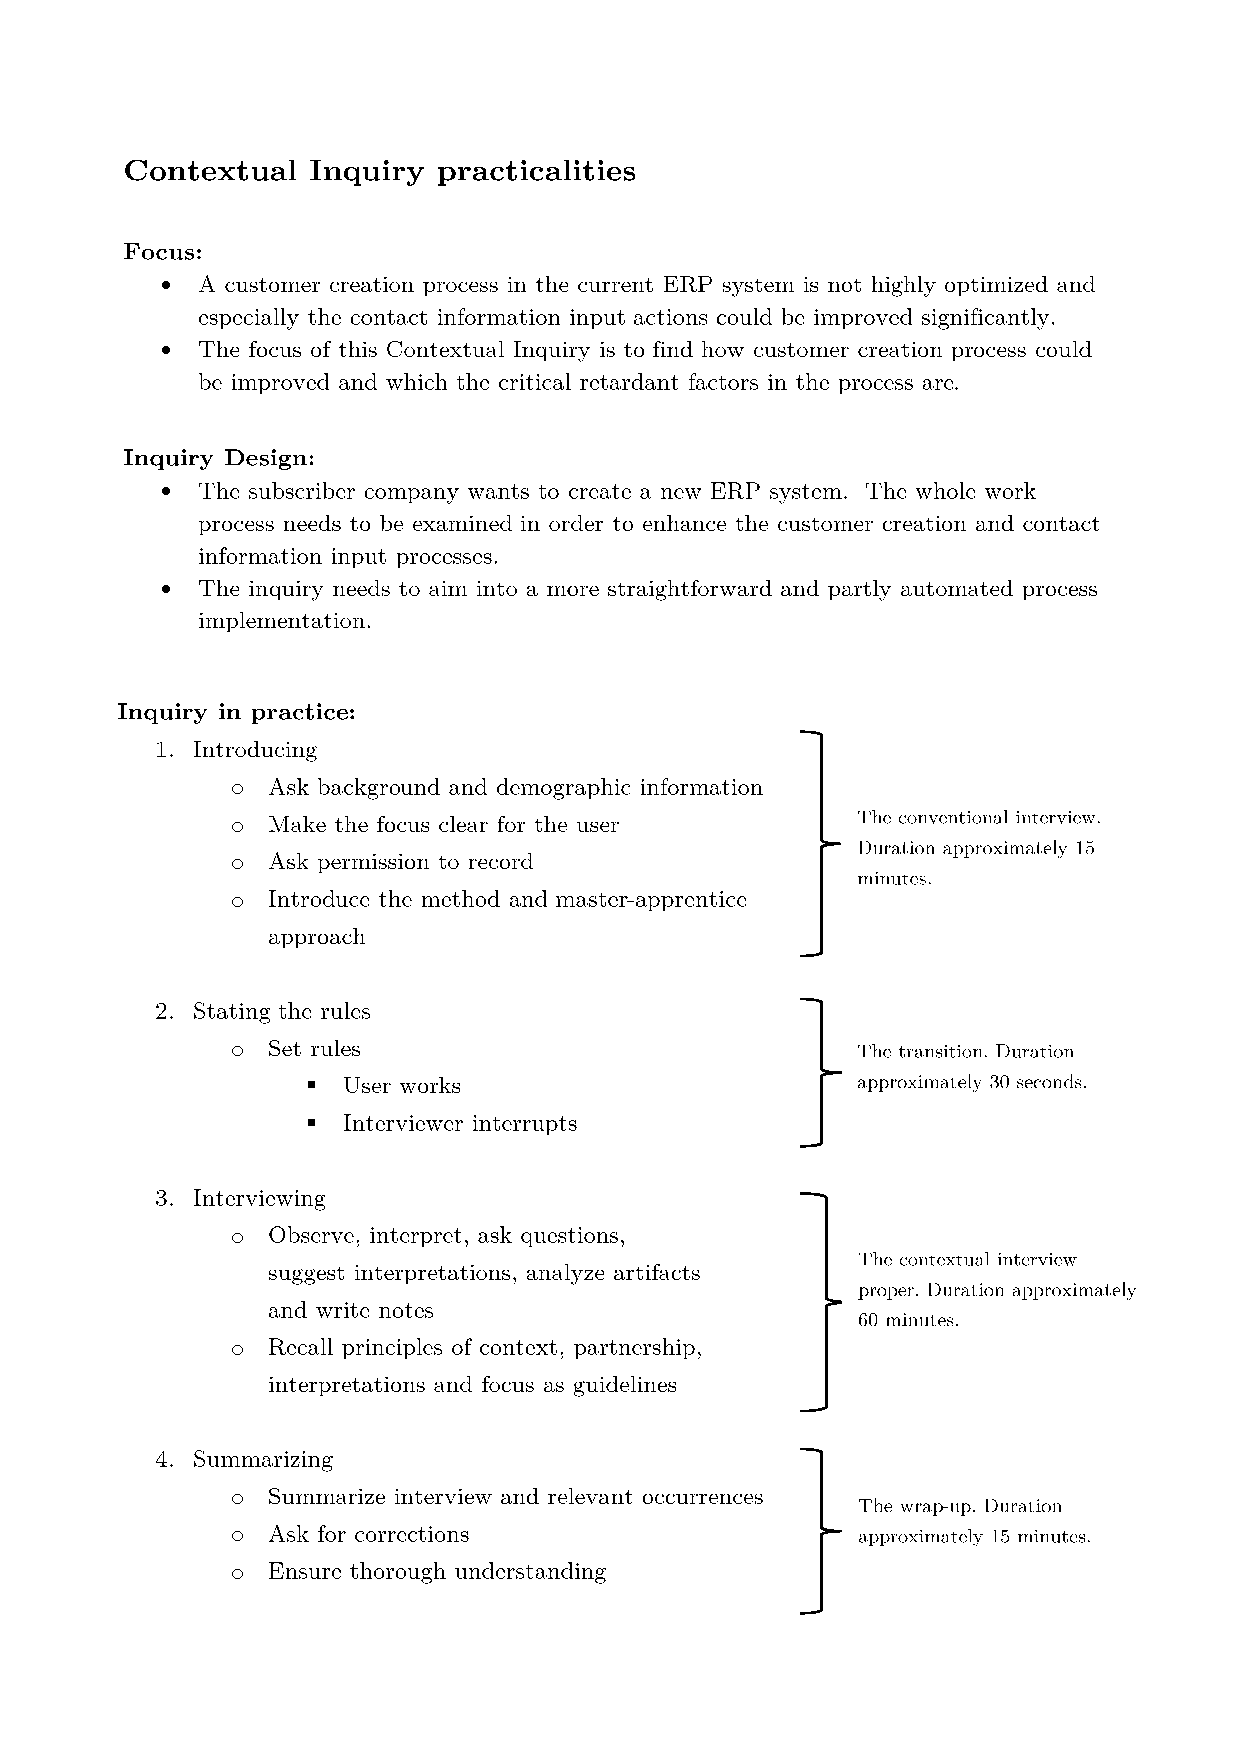
\includepdf[scale=0.85,pages=1,angle=0.0,picturecommand*={%
     \put(95,780){%
         \parbox{\textwidth}{\chapter{Contextual Inquiry: Research plan}\label{app:ciresearch}}
     }}]{./pdfs/ciplan.pdf}



%\includepdf[scale=0.9,pages=4,picturecommand*={%
%     \put(110,770){%
%         \parbox{\textwidth}{\chapter{TEST form}\label{app:susform}}
%     }}]{sus.pdf}


%\includegraphics[scale=0.5,pages={4}]{sus.pdf}

%\includepdf[ pages=4, scale=.7, frame, pagecommand =  \chapter{}]{sus.pdf}
%\chapter{}
%\includegraphics[page=4,width=1.2\textwidth]{sus.pdf}
%\chapter{SUS form}
%\label{chapter:susform}
%\begin{figure}[h]
 %  \centering
   %\begin{tabular}{@{}c@{\vspace{2.5cm}}c@{}}
      % \includegraphics[page=4,width=1.2\textwidth]{sus.pdf} & 

   %\end{tabular}
 %\label{fig:Test}
%\end{figure}



%    \section{APPENDIX A}
%    \label{sec:appendixa}
%This is the first appendix. You could put some test images or verbose data in an
%appendix, if there is too much data to fit in the actual text nicely.

%For now, the Aalto logo variants are shown in Figure~\ref{fig:aaltologo}.

%\begin{figure}
%\begin{center}
%\subfigure[In English]{
\includegraphics[width=.8\textwidth]{aalto-logo-en}}
%\subfigure[Suomeksi]{
\includegraphics[width=.8\textwidth]{aalto-logo-fi}}
%\subfigure[Pä svenska]{
\includegraphics[width=.8\textwidth]{aalto-logo-se}}
%\caption{Aalto logo variants}
%\label{fig:aaltologo}
%\end{center}
%\end{figure}


% End of document!
% ------------------------------------------------------------------
% The LastPage package automatically places a label on the last page.
% That works better than placing a label here manually, because the
% label might not go to the actual last page, if LaTeX needs to place
% floats (that is, figures, tables, and such) to the end of the
% document.
\end{document}
